\setcounter{chapter}{4}

\chapter{Variable Selection}

{\small \textit{Chapter Preview}. This chapter describes tools and
techniques to help you select variables to enter into a linear
regression model, beginning with an iterative model selection
process. In applications with many potential explanatory variables,
automatic variable selection procedures are available that will help
you quickly evaluate many models. Nonetheless, automatic procedures
have serious limitations including the inability to account properly
for nonlinearities such as the impact of unusual points; this
chapter expands upon the Chapter 2 discussion of unusual points. It
also describes collinearity, a common feature of regression data
where explanatory variables are linearly related to one another.
Other topics that impact variable selection, including
heteroscedasticity and out-of-sample validation, are also
introduced.}

\section{An Iterative Approach to Data Analysis and
Modeling}\label{S5:Iterative}

In our introduction of basic linear regression in Chapter 2, we
examined the data graphically, hypothesized a model structure, and
compared the data to a candidate model in order to formulate an
improved model. Box (1980) describes this as an \emph{iterative
process} which is shown in Figure \ref{F5:Iterative}.


\begin{figure}[htp]
    \includegraphics[width=1\textwidth,angle=270,scale=0.5]{Chapter5/F5Iterative.ps}
   \caption{\label{F5:Iterative} \small The iterative model specification process.}
\end{figure}

\marginparjed{Diagnostic checking reflects symptoms of mistakes made
in previous specification steps and provides ways to correct these
mistakes.}


This iterative process provides a useful recipe for structuring the
task of specifying a model to represent a set of data. The first
step, the model formulation stage, is accomplished by examining the
data graphically and using prior knowledge of relationships, such as
from economic theory or standard industry practice. The second step
in the iteration is based on the assumptions of the specified model.
These assumptions must be consistent with the data to make valid use
of the model. The third step, \emph{diagnostic checking}, is also
known as \emph{data and model criticism}; the data and model must be
consistent with one another before additional inferences can be
made. Diagnostic checking is an important part of the model
formulation; it can reveal mistakes made in previous steps and
provide ways to correct these mistakes.

The iterative process also emphasizes the skills you need to make
regression analysis work. First, you need a willingness to summarize
information numerically and portray this information graphically.
Second, it is important to develop an understanding of model
properties. You should understand how a theoretical model behaves in
order to match a set of data to it. Third, theoretical properties of
the model are also important for inferring general relationships
based on the behavior of the data.


\section{Automatic Variable Selection
Procedures}\label{S5:Automatic}

Business and economics relationships are complicated, there are
generally many variables that could serve as useful predictors of
the response. In searching for a suitable model, there is a large
number of potential models that are based on linear combinations of
explanatory variables and an infinite number that can be formed from
nonlinear combinations. To search among models based on linear
combinations, several automatic procedures are available to select
variables to be included in the model. These automatic procedures
are easy to use and will suggest one or more models that you can
explore in further detail.

To illustrate how large is the potential number of linear models,
suppose that there are only four variables, $x_{1},$ $x_2,$ $x_3$
and $x_4$, under consideration for fitting a model to $y$. Without
any consideration of multiplication or other nonlinear combinations
of explanatory variables, how many possible models are there? Table
\ref{T5:NumberModels} shows that the answer is 16.

\begin{table}[h]
\scalefont{0.9}

\caption{\label{T5:NumberModels} Sixteen Possible Models}
\begin{tabular}{llll}
\hline
E $y=\beta_0$ &  &  & 1 model with no independent \\
&  &  & \ \ variables \\
E $y=\beta_0+\beta_1x_i,$ & $i=$ & $1,2,3,4$ & 4 models with one
independent \\
&  &  & \ \ variable \\
E $y = \beta_0 + \beta_1 x_i + \beta_2 x_j,$ & $(i,j)=$ & $
(1,2),(1,3),(1,4),$ & 6 models with two independent \\
&  & $(2,3),(2,4),(3,4)$ & \ \ variables \\
E $y = \beta_0 + \beta_1 x_1 + \beta_2 x_j$ & $(i,j,k)=$ & $
(1,2,3),(1,2,4),$ & 4 models with three independent \\
$\ \ \ \ \ \ \ \ +\beta_3x_{k},$ &  & $(1,3,4),(2,3,4)$ & \ \
variables
\\
E $y = \beta_0 + \beta_1 x_1 + \beta_2 x_2$ &  &  & 1 model with all
independent \\
$\ \ \ \ \ \ \ \ +\beta_3 x_3 + \beta_4 x_4$ &  &  & \ \ variables \\
\hline
\end{tabular}
\scalefont{1.1111}
\end{table}


\noindent If there were only three explanatory variables, then you
can use the same logic to verify that there are eight possible
models. Extrapolating from these two examples, how many linear
models will there be if there are ten explanatory variables? The
answer is 1,024, which is quite a few. In general, the answer is
$2^k$, where $k$ is the number of explanatory variables. For
example, $2^3$ is 8, $2^4$ is 16, and so on.

In any case, for a moderately large number of explanatory variables,
there are many potential models that are based on linear
combinations of explanatory variables. We would like a procedure to
search quickly through these potential models to give us more time
to think about other interesting aspects of model selection. One
procedure for bringing explanatory variables into the model is
\textit{stepwise regression}. This procedure employs a series of
\textit{t}-tests to check the ``significance'' of explanatory
variables entered into, or deleted from, the model. The following is
a description of the basic algorithm.

\bigskip

\boxedjed
\subsubsection*{Stepwise Regression Algorithm}

Suppose that the analyst has identified one variable as the
response, $y$, and $k$ potential explanatory variables, $x_1, x_2,
\ldots, x_k$.
\begin{enumerate}

\item Consider all possible regressions using one explanatory variable.
For each of the $k$ regressions, compute $t(b_1)$, the $t$-ratio for
the slope. Choose that variable with the largest $t$-ratio. If the
\textit{t}-ratio does not exceed a pre-specified $t$-value (such as
two), then do not choose any variables and halt the procedure.

\item Add a variable to the model from the previous step. The variable to enter
is the one that makes the largest significant contribution. To
determine the
size of contribution, use the absolute value of the variable's \textit{t}%
-ratio. To enter, the $t$-ratio must exceed a specified $t$-value in
absolute value.

\item Delete a variable to the model from the previous step. The variable to be
removed is the one that makes the smallest contribution. To
determine the size of contribution, use the absolute value of the
variable's $t$-ratio. To be removed, the $t$-ratio must be less than
a specified $t$-value in absolute value.

\item Repeat steps (ii) and (iii) until all possible additions and deletions are
performed.
\end{enumerate}

\end{boxedminipage}

\bigskip


\noindent When implementing this routine, some statistical software
packages use an \textit{F-}test in lieu of $t$-tests. Recall, when
only one variable is being considered, that ($t$-ratio)$^{2}$ =
\textit{F-}ratio and thus these procedures are equivalent.

This algorithm is useful in that it quickly searches through a number of
candidate models. However, there are several drawbacks:
\begin{enumerate}

\item The procedure ``snoops'' through a large number of models and may
fit the data ``too well.''

\item There is no guarantee that the selected model is the best. The algorithm
does not consider models that are based on nonlinear combinations of
explanatory variables. It also ignores the presence of outliers and
high leverage points. \index{leverage}\index{outlier}

  \item In addition, the algorithm does not even search all $2^{k}$ possible
linear regressions.

  \item The algorithm uses one criterion, a \textit{t}-ratio, and does not
consider other criteria such as s, $R^2$, R, and so on.

  \item There is a sequence of significance tests involved. Thus, the
significance level that determines the \textit{t}-value is not
meaningful.

  \item By considering each variable separately, the algorithm does not take into
account the joint effect of explanatory variables.

  \item Purely automatic procedures may not take into account an investigator's
special knowledge.

\end{enumerate}

Simpler variants of the algorithm are available. An advantage of
these variants is that they are easier to explain and
computationally simpler (important for large data sets). These
include:

\begin{itemize}
\item Forward selection. Add one variable at a time without trying
to delete variables.

\item Backwards selection. Start with the full model and delete one variable at
a time without trying to add variables.

\end{itemize}

Many of the criticisms of the basic stepwise regression algorithm
can be addressed with modern computing software that is now widely
available. We now consider each drawback, in reverse order. To
respond to drawback number (vii), many statistical software routines
have options for forcing variables into a model equation. In this
way, if other evidence indicates that one or more variables should
be included in the model, then the investigator can force the
inclusion of these variables.

For drawback number (vi), in Section \ref{S5:Suppressor} on
\textit{suppressor variables}, we will provide examples of variables
that do not have important individual effects but are important when
considered jointly. These combinations of variables may not be
detected with the basic algorithm but will be detected with the
backwards selection algorithm. Because the backwards procedure
starts with all variables, it will detect, and retain, variables
that are jointly important.

Drawback number (v) is really a suggestion about the way to use
stepwise regression. Bendel and Afifi (1977) suggested using a
cut-off smaller than you ordinarily might. For example, in lieu of
using \textit{t}-value = 2 corresponding approximately to a 5\%
significance level, consider using \textit{t}-value = 1.645
corresponding approximately to a 10\% significance level. In this
way, there is less chance of screening out variables that may be
important. A lower bound, but still a good choice for exploratory
work, is a cut-off as small as \textit{t}-value = 1. This choice is
motivated by an algebraic result: when a variable enters a model,
$s$ will decrease if the \textit{t}-ratio exceeds one in absolute
value.

\marginparjed{When a variable enters a model, $s$ will decrease if
the \textit{t}-ratio exceeds one in absolute value.}

To address drawbacks number (iii) and (iv), we now introduce the \textit{%
best regressions }routine. Best regressions is a useful algorithm that is
now widely available in statistical software packages. The best regression
algorithm searches over all possible combinations of explanatory variables,
unlike stepwise regression, that adds and deletes one variable at a time.
For example, suppose that there are four possible explanatory variables, $%
x_1$, $x_2$, $x_3$ and $x_4$, and the user would like to know what
is the best two variable model. The best regression algorithm
searches over all six models of the form E $y$ = $\beta_0$ +
$\beta_1$ $x_i$ + $\beta_2$ $x_j$. Typically, a best regression
routine recommends one or two models for each $p$ coefficient model,
where \textit{p} is a number that is user specified. Because it has
specified the number of coefficients to enter the model, it does not
matter which of the criteria we use: $R^2$, $R$, or $s$.

The best regression algorithm performs its search by a clever use of
the algebraic fact that, when a variable is added to the model, the
error sum of squares does not increase. Because of this fact,
certain combinations of variables included in the model need not be
computed. An important drawback of this algorithm is that it can
take a considerable amount of time when the number of variables
considered is large.

Users of regression do not always appreciate the depth of drawback
number (i), \textit{data-snooping}. Data-snooping occurs when the
analyst fits a great number of models to a data set. We will address
the problem of data-snooping in Section \ref{S5:ModelValidation} on
model validation. Here, we illustrate the effect of data-snooping in
stepwise regression.

\linejed

\textbf{Example: Data-Snooping in Stepwise
Regression.}\ecaptionjed{Data-Snooping in Stepwise Regression} The
idea of this illustration is due to Rencher and Pun (1980). Consider
$n=100$ observations of $y$ and fifty explanatory variables, $x_1,
x_2, \ldots,x_{50}$. The data we consider here were simulated using
independent standard normal random variates. Because the variables
were simulated independently, we are working under the null
hypothesis of no relation between the response and the explanatory
variables, that is, H$_0$: $\beta_1=\beta_2=$ $\ldots$
$=\beta_{50}=0$. Indeed, when the model with all
fifty explanatory variables was fit, it turns out that $s=1.142$, $%
R^2=46.2\%$ and \textit{F-}ratio = (Regression MS) / (Error MS) =
0.84. Using an \textit{F-}distribution with $df_1=50$ and $df_2=49$,
the 95th percentile is 1.604. In fact, 0.84 is the 27th percentile
of this distribution, indicating that the \textit{p-}value is 0.73.
Thus, as expected, the data are in congruence with $H_0$.

Next, a stepwise regression with \textit{t}-value = 2 was performed. Two
variables were retained by this procedure, yielding a model with $s=1.05$, $%
R^2=9.5\%$ and \textit{F-}ratio = 5.09. For an
\textit{F-}distribution with $df_1=2$ and $df_2=97$, the 95th
percentile is \textit{F-}value = 3.09. This indicates that the two
variables are statistically significant predictors of $y$. At first
glance, this result is surprising. The data were generated so
that $y$ is unrelated to the explanatory variables. However, because \textit{%
F-}ratio $>$ \textit{F-}value, the \textit{F-}test indicates that
two explanatory variables are significantly related to $y$. The
reason is that stepwise regression has performed many hypothesis
tests on the data. For example, in Step 1, fifty tests were
performed to find significant variables. Recall that a 5\% level
means that we expect to make roughly one mistake in 20. Thus, with
fifty tests, we expect to find $50(0.05)=2.5$ ``significant''
variables, even under the null hypothesis of no relationship between
$y$ and the explanatory variables.

To continue, a stepwise regression with \textit{t-}value = 1.645 was
performed. Six variables were retained by this procedure, yielding a
model with $s=0.99$, $R^2=22.9\%$ and \textit{F-}ratio = 4.61. As
before, an \textit{F-}test indicates a significant relationship
between the response and these six explanatory variables.

\marginparjed{When explanatory variables are selected using the
data, \textit{t-}ratios and \textit{F-}ratios will be too large,
thus overstating the importance of variables in the model.}

To summarize, using simulation we constructed a data set so that the
explanatory variables have no relationship with the response.
However, when using stepwise regression to examine the data, we
``found'' seemingly significant relationships between the response
and certain subsets of the explanatory variables. This example
illustrates a general caveat in model selection: when explanatory
variables are selected using the data, \textit{t-}ratios and
\textit{F-}ratios will be too large, thus overstating the importance
of variables in the model.

\linejed

\newpage

\marginparjed{A model suggested by automatic variable selection
procedures should be subject to the same careful diagnostic checking
procedures as a model arrived at by any other means.}

Stepwise regression and best regressions are examples of
\textit{automatic variable selection procedures}. In your modeling
work, you will find these procedures to be useful because they can
quickly search through several candidate models. However, these
procedures do ignore nonlinear alternatives as well as the effect of
outliers and high leverage points. The main point of the procedures
is to mechanize certain routine tasks. This automatic selection
approach can be extended and indeed, there are a number of so-called
``expert systems'' available in the market. For example, algorithms
are available that ``automatically'' handle unusual points such as
outliers and high leverage points. A model suggested by automatic
variable selection procedures should be subject to the same careful
diagnostic checking procedures as a model arrived at by any other
means. \index{leverage}\index{outlier}

\section{Residual Analysis}\label{S5:ResidualAnalysis}

Recall the role of a residual in the linear regression model
introduced in Section 2.6. A residual is a response minus the
corresponding fitted value under the model. Because the model
summarizes the linear effect of several explanatory variables, we
may think of a residual as a response controlled for values of the
explanatory variables. If the model is an adequate representation of
the data, then residuals should closely approximate random errors.
Random errors are used to represent the natural variation in the
model; they represent the result of an unpredictable mechanism.
Thus, to the extent that residuals resemble random errors, there
should be no discernible patterns in the residuals. Patterns in the
residuals indicate the presence of additional information that we
hope to incorporate into the model. A lack of patterns in the
residuals indicates that the model seems to account for the primary
relationships in the data.

\marginparjed{Patterns in the residuals indicate the presence of
additional information that we hope to incorporate into the model. A
lack of patterns in the residuals indicates that the model seems to
account for the primary relationships in the data.}

\subsection{Residuals}\label{S5:Residuals}

There are at least four types of patterns that can be uncovered
through the residual analysis. In this section, we discuss the first
two; residuals that are unusual and those that are related to other
explanatory variables. We then introduce the third type, residuals
that display a heteroscedastic pattern, in Section
\ref{S5:Heteroscedasticity}. In our study of time series data that
begins in Chapter 7, we will introduce the fourth type, residuals
that display patterns through time.\index{heteroscedasticity}

When examining residuals, it is usually easier to work with a \textit{%
standardized residual}, a residual that has been rescaled to be
dimensionless. We generally work with standardized residuals because
we achieve some carry-over of experience from one data set to
another and may thus focus on relationships of interest. By using
standardized residuals, we can train ourselves to look at a variety
of residual plots and immediately recognize an unusual point when
working in standard units.

There are a number of ways of defining a standardized residual.
Using $e_i = y_i-\hat{y}_i$ as the $i$th residual, here are three
commonly used definitions:

\begin{equation} \label{E5:StdResid}
\text{(a) }\frac{e_i}{s},\text{ \ \ \ (b) }\frac{e_i}{s\sqrt{
1-h_{ii}}}, \text { \  \   \   }\text{(c)
}\frac{e_i}{s_{(i)}\sqrt{1-h_{ii}}}\text{\ }.
\end{equation}
\index{leverage} \noindent Here, $h_{ii}$ is the $i$th leverage. It
is calculated based on values of the explanatory variables and will
be defined in Section \ref{S5:Leverage}. Recall that $ s $ is the
residual standard deviation (defined in equation 3.8). Similarly,
define $s_{(i)}$ to be the residual standard deviation when running
a regression after having deleted the $i$th observation.

Now, the first definition in (a) is simple and easy to explain. An
easy calculation shows that the sample standard deviation of the
residuals is approximately $s$ (one reason that $s$ is often
referred to as the residual standard deviation). Thus, it seems
reasonable to standardize residuals by dividing by $s$.

The second choice presented in (b), although more complex, is more
precise. The variance of the $i$th residual is
\begin{equation*}
\mathrm{Var}(e_i)=\sigma ^2(1-h_{ii}).
\end{equation*}
This result will be established in equation \ref{E5:VarResiduals} of
Section \ref{S5:TechSupps}. Note that this variance is smaller than
the variance of the error term, Var $(\varepsilon_i)=\sigma ^2$.
Now, we can replace $\sigma $ by its estimate, $s$. Then, this
result leads to using the quantity $s(1-h_{ii})^{1/2}$ as an
estimated standard deviation, or standard error, for $e_i$. Thus, we
define the standard error of $e_i$ to be
\begin{equation*}
se(e_i)=s \sqrt{1-h_{ii}}.
\end{equation*}
Following the conventions introduced in Section 2.6, in this text we
use $e_i/se(e_i)$ to be our \textit{standardized residual}.

The third choice presented in (c) is a modification of (b) and is
known as a \textit{studentized residual}. As emphasized in Section
\ref{S5:ResidualsOutliers}, one important use of residuals is to
identify unusually large responses. Now, suppose that the $i$th
response is unusually large and that this is measured through its
residual. This unusually large residual will also cause the value of
$s$ to be large. Because the large effect appears in both the
numerator and denominator, the standardized residual may not detect
this unusual response. However, this large response will not inflate
$s_{(i)}$ because it is constructed after having deleted the $i$th
observation. Thus, when using studentized residuals we get a better
measure of observations that have unusually large residuals. By
omitting this observation from the estimate of $\sigma $, the size
of the observation affects only the numerator $e_i$ and not the
denominator $s_{(i)}$.\index{outlier}

As another advantage, studentized residuals follow a
\textit{t-}distribution with $n-(k+1)$ degrees of freedom, assuming
the errors are normally distributed (assumption E5). This knowledge
of the precise distribution helps us assess the degree of model fit,
and is particularly useful in small samples. It is this relationship
with the ``Student's'' \textit{t-}distribution that suggests the
name ``studentized'' residuals.

\subsection{Using Residuals to Identify
Outliers}\label{S5:ResidualsOutliers}\index{outlier}

\marginparjed{A commonly used rule of thumb is to mark an
observation as an outlier if its' standardized residual exceeds two
in absolute value.}

One important role of residual analysis is to identify outliers. An
outlier is an observation that is not well fit by the model; these
are observations where the residual is unusually large. A rule of
thumb that is used by many statistical packages is that an
observation is marked as an outlier if the standardized residual
exceeds two in absolute value. To the extent that the distribution
of standardized residuals mimics the standard normal curve, we
expect about only one in 20 observations, or 95\%, to exceed two in
absolute value and very few observations to exceed three.

Outliers provide a signal that an observation should be investigated
to understand special causes associated with this point. An outlier
is an observation that seems unusual with respect to the rest of the
data set. It is often the case that the reason for this atypical
behavior may be uncovered after additional investigation. Indeed,
this may be the primary purpose of the regression analysis of a data
set.

Consider a simple example of so-called \textit{performance
analysis}. Suppose we have available a sample of $n$ salespeople and
are trying to understand each person's second-year sales based on
their first-year sales. To a certain extent, we expect that higher
first-year sales are associated with higher second-year sales. High
sales may be due to a salesperson's natural ability, ambition, good
territory, and so on. First-year sales may be thought of as a proxy
variable that summarizes these factors. We expect variation in sales
performance both cross-sectionally and across years. It is
interesting when one salesperson performs unusually well (or poorly)
in the second year compared to their first-year performance.
Residuals provide a formal mechanism for evaluating second-year
sales after controlling for the effects of first-year sales.

There are a number of options available for handling outliers.

\bigskip

\boxedjed

\textit{Options for Handling Outliers}
\begin{itemize}
\item  Include the observation in
the usual summary statistics but comment on its effects. An outlier
may be large but not so large as to skew the results of the entire
analysis. If no special causes for this unusual observation can be
determined, then this observation may simply reflect the variability
in the data.

\item  Delete the observation from the data set. The observation may be
determined to be unrepresentative of the population from which the
sample is drawn. If this is the case, then there may be little
information contained in the observation that can be used to make
general statements about the population. This option means that we
would omit the observation from the regression summary statistics
and discuss it in our report as a separate case.

\item  Create a binary variable to indicate the presence of an outlier. If one or several
special causes have been identified to explain an outlier, then
these causes could be introduced into the modeling procedure
formally by introducing a variable to indicate the presence (or
absence) of these causes. This approach is similar to point deletion
but allows the outlier to be formally included in the model
formulation so that, if additional observations arise that are
affected by the same causes, then they can be handled on an
automatic basis.

\end{itemize}

\end{boxedminipage}

\bigskip

\subsection{Using Residuals to Select Explanatory
Variables}\label{S5:ResidualsExplanatory}

Another important role of residual analysis is to help identify
additional explanatory variables that may be used to improve the
formulation of the model. If we have specified the model correctly,
then residuals should resemble random errors and contain no
discernible patterns. Thus, when comparing residuals to explanatory
variables, we do not expect any relationships. If we do detect a
relationship, then this suggests the need to control for this
additional variable. This can be accomplished by introducing the
additional variable into the regression model.

Relationships between residuals and explanatory variables can be
quickly established using correlation statistics. However, if an
explanatory variable is already included in the regression model,
then the correlation between the residuals and an explanatory
variable will be zero (Section \ref{S5:ProjMatrix} provides the
algebraic demonstration). It is a good idea to reinforce this
correlation with a scatter plot. Not only will a plot of residuals
versus explanatory variables reinforce graphically the correlation
statistic, it will also serve to detect potential nonlinear
relationships. For example, a quadratic relationship can be detected
using a scatter plot, not a correlation statistic.

If you detect a relationship between the residuals from a
preliminary model fit and an additional explanatory variable, then
introducing this additional variable will not always improve your
model specification. The reason is that the additional variable may
be linearly related to the variables that are already in the model.
If you would like a guarantee that adding an additional variable
will improve your model, then construct an added variable plot (from
Section 3.4.3). \index{added variable plot}

To summarize, after a preliminary model fit, you should:
\begin{itemize}
\item Calculate summary statistics and display the distribution of
(standardized) residuals to identify outliers.\index{outlier}

\item  Calculate the correlation between the (standardized) residuals and
additional explanatory variables to search for linear relationships.

\item  Create scatter plots between the (standardized) residuals and additional
explanatory variables to search for nonlinear relationships.
\end{itemize}

\linejed

\textbf{Example: Stock Liquidity.}\ecaptionjed{Stock Liquidity} An
investor's decision to purchase a stock is generally made with a
number of criteria in mind. First, investors usually look for a high
expected return. A second criterion is the riskiness of a stock
which can be measured through the variability of the returns. Third,
many investors are concerned with the length of time that they are
committing their capital with the purchase of a security. Many
income stocks, such as utilities, regularly return portions of
capital investments in the form of dividends. Other stocks,
particularly growth stocks, return nothing until the sale of the
security. Thus, the average length of investment in a security is
another criterion. Fourth, investors are concerned with the ability
to sell the stock at any time convenient to the investor. We refer
to this fourth criterion as the \textit{liquidity }of the stock. The
more liquid is the stock, the easier it is to sell. To measure the
liquidity, in this study we use the number of shares traded on an
exchange over a specified period of time (called the VOLUME). We are
interested in studying the relationship between the volume and other
financial characteristics of a stock.

We begin this study with 126 companies whose options were traded on December
3, 1984. The stock data were obtained from Francis Emory Fitch, Inc. for the
period from December 3, 1984 to February 28, 1985. For the trading activity
variables, we examine
\begin{itemize}
\item the three months total trading volume (VOLUME, in millions of shares),
\item the three months total number of transactions (NTRAN), and
\item the average time between transactions (AVGT, measured in minutes).
\end{itemize}
\noindent For the firm size variables, we use the
\begin{itemize}
\item opening stock price on January 2, 1985 (PRICE),
\item  the number of outstanding shares on December 31, 1984 (SHARE, in millions of shares), and
\item  the market equity value (VALUE, in billions of dollars) obtained by taking the product of PRICE and SHARE.
\end{itemize}
\noindent Finally, for the financial leverage, we examine the
debt-to-equity ratio (DEB\_EQ) obtained from the Compustat
Industrial Tape and the Moody's manual. The data in SHARE are
obtained from the Center for Research in Security Prices (CRSP)
monthly tape.

After examining some preliminary summary statistics of the data,
three companies were deleted because they either had an unusually
large volume or high price. They are Teledyne and Capital Cities
Communication, whose prices were more than four times the average
price of the remaining companies, and American Telephone and
Telegraph, whose total volume was more than seven times than the
average total volume of the remaining companies. Based on additional
investigation, the details of which are not presented here, these
companies were deleted because they seemed to represent special
circumstances that we would not wish to model. Table
\ref{T5:LiquidSumStats} summarizes the descriptive statistics based
on the remaining $n=123$ companies. For example, from Table
\ref{T5:LiquidSumStats} we see that the average time between
transactions is about five minutes and this time ranges from a
minimum of less than a minute to a maximum of about 20 minutes.

\begin{table}[h]
\scalefont{0.9}

\caption{\label{T5:LiquidSumStats} Summary Statistics of the Stock
Liquidity Variables}

\begin{tabular}{lrrrrr}
\hline
&  & & Standard &  &  \\
& Mean & Median & deviation & Minimum & Maximum \\
\hline VOLUME & 13.423 & 11.556 & 10.632 &
0.658 & 64.572 \\
AVGT & 5.441 & 4.284 & 3.853 & 0.590 &
20.772 \\
NTRAN & 6436 & 5071 & 5310 & 999 &
36420 \\
PRICE & 38.80 & 34.37 & 21.37 & 9.12 &
122.37 \\
SHARE & 94.7 & 53.8 & 115.1 & 6.7 &
783.1 \\
VALUE & 4.116 & 2.065 & 8.157 & 0.115 &
75.437 \\
DEB\_EQ & 2.697 & 1.105 & 6.509 & 0.185 & 53.628 \\ \hline
\end{tabular}

\textit{Source: Francis Emory Fitch, Inc., Standard \& Poor's
Compustat, and University of Chicago's Center for Research on
Security Prices.}

\scalefont{1.1111}
\end{table}

Table \ref{T5:LiquidCorr} reports the correlation coefficients and
Figure \ref{F5:LiquidPlot} provides the corresponding scatterplot
matrix. If you have a background in finance, you will find it
interesting to note that the financial leverage, measured by
DEB\_EQ, does not seem to be related to the other variables. From
the scatterplot and correlation matrix, we see a strong relationship
between VOLUME and the size of the firm as measured by SHARE and
VALUE. Further, the three trading activity variables, VOLUME, AVGT
and NTRAN, are all highly related to one another.

\begin{table}[h]
\scalefont{0.9}

\caption{\label{T5:LiquidCorr} Correlation Matrix of the Stock
Liquidity}
\begin{tabular}{lrrrrrrr}
\hline & AVGT & NTRAN & PRICE & SHARE & VALUE & DEB\_EQ \\ \hline
\multicolumn{1}{l}{NTRAN} & $-0.668$ &  &  &  &  &  \\
\multicolumn{1}{l}{PRICE} & $-0.128$ & $0.190$ &  &  &  &  \\
\multicolumn{1}{l}{SHARE} & $-0.429$ & $0.817$ & $0.177$ &  &  &  \\
\multicolumn{1}{l}{VALUE} & $-0.318$ & $0.760$ & $0.457$ & $0.829$ &  &  \\
\multicolumn{1}{l}{DEB\_EQ} & $0.094$ & $-0.092$ & $-0.038$ & $-0.077$ & $%
-0.077$ &  \\
\multicolumn{1}{l}{VOLUME} & $-0.674$ & $0.913$ & $0.168$ & $0.773$ & $0.702$
& $-0.052$ \\ \hline
\end{tabular}
\scalefont{1.1111}
\end{table}

Figure \ref{F5:LiquidPlot} shows that the variable AVGT is inversely
related to VOLUME and NTRAN is inversely related to AVGT. In fact,
it turned out the correlation between the average time between
transactions and the reciprocal of the number of transactions was
$99.98\%$! This is not so surprising when one thinks about how AVGT
might be calculated. For example, on the New York Stock Exchange,
the market is open from 10:00 A.M. to 4:00 P.M. For each stock on a
particular day, the average time between transactions times the
number of transactions is nearly equal to 360 minutes (= 6 hours).
Thus, except for rounding errors because transactions are only
recorded to the nearest minute, there is a perfect linear
relationship between AVGT and the reciprocal of NTRAN.


\begin{figure}[htp]
  \begin{center}
    \includegraphics[width=1\textwidth,angle=270,scale=0.75]{Chapter5/F5LiquidPlot.ps}
    \caption{\label{F5:LiquidPlot} \small  Scatterplot matrix for
stock liquidity variables. The number of transactions variable
(NTRAN) appears to be strongly related to the VOLUME of shares
traded, and inversely related to AVGT.}
  \end{center}
\end{figure}


To begin to understand the liquidity measure VOLUME, we first fit a
regression model using NTRAN as an explanatory variable. The fitted
regression model is:

\scalefont{0.9}
\begin{center}
\begin{tabular}{lccl}
  VOLUME & = & 1.65 & +0.00183 NTRAN \\
  std errors &  & (0.0018)  & (0.000074) \\
\end{tabular}
\end{center}
\scalefont{1.1111}

\noindent with $R^2=83.4\%$ and $s=4.35$. Note that the
\textit{t-}ratio for the slope associated with NTRAN is
$t(b_1)=b_1/se(b_1)=0.00183/0.000074=24.7$, indicating strong
statistical significance. Residuals were computed using this
estimated model. To see if the residuals are related to the other
explanatory variables, below is a table of correlations.


\begin{table}[h]
\scalefont{0.9}

\caption{\label{T5:LiquidResidCorr1} First Table of Correlations }
\begin{tabular}{cccccc}
 \hline
& AVGT & PRICE & SHARE & VALUE & DEB\_EQ \\
RESID & -0.155 & -0.017 & 0.055 & 0.007 & 0.078 \\ \hline
\end{tabular}

{\small \textit{Note:} The residuals were created from a regression
of VOLUME on NTRAN.} \scalefont{1.1111}
\end{table}

The correlation between the residual and AVGT and the scatter plot (not
given here) indicates that there may be some information in the variable
AVGT in the residual. Thus, it seems sensible to use AVGT directly in the
regression model. Remember that we are interpreting the residual as the
value of VOLUME having controlled for the effect of NTRAN.

We next fit a regression model using NTRAN and AVGT as an explanatory
variables. The fitted regression model is:

\scalefont{0.9}
\begin{center}
\begin{tabular}{lccll}
  VOLUME     & = & 4.41   & -0.322 AVGT & +0.00167 NTRAN \\
  std errors &   & (1.30) & (0.135)     & (0.000098)     \\
\end{tabular}
\end{center}
\scalefont{1.1111}


\noindent with $R^2=84.2\%$ and $s=4.26$. Based on the
\textit{t-}ratio for AVGT, $t(b_{AVGT})=$ $(-0.322)/0.135$ $=-2.39$,
it seems as if AVGT is a useful explanatory variable in the model.
Note also that $s$ has decreased, indicating that $R_a^2$ has
increased.

Table \ref{T5:LiquidResidCorr2} provides correlations between the
model residuals and other potential explanatory variables and
indicates that there does not seem to be much additional information
in the explanatory variables. This is reaffirmed by the
corresponding table of scatter plots in Figure
\ref{F5:LiquidResidPlot}. The histograms in Figure
\ref{F5:LiquidResidPlot} suggest that although the distribution of
the residuals is fairly symmetric, the distribution of each
explanatory variable is skewed. Because of this, transformations of
the explanatory variables were explored. This line of thought
provided no real improvements and thus the details are not provided
here.

\begin{figure}[htp]
  \begin{center}
    \includegraphics[width=1\textwidth,angle=270,scale=0.5]{Chapter5/F5LiquidResidPlot.ps}
    \caption{\label{F5:LiquidResidPlot} \small  Scatterplot matrix of the
residuals from the regression of VOLUME on NTRAN and AVGT on the
vertical axis and the remaining predictor variables on the
horizontal axes.}
  \end{center}
\end{figure}



\begin{table}[h]
\scalefont{0.9}

\caption{\label{T5:LiquidResidCorr2} Second Table of Correlations }
\begin{tabular}{ccccc}
\hline
& PRICE & SHARE & VALUE & DEB\_EQ \\
RESID & -0.015 & 0.096 & 0.071 & 0.089 \\ \hline
\end{tabular}

{\small \textit{Note:} The residuals were created from a regression
of VOLUME on NTRAN and AVGT.} \scalefont{1.1111} \scalefont{1.1111}
\end{table}

\linejed

\section{Influential Points}

Not all points are created equal -- in this section we will see that
specific observations can have a disproportionate effect on the
overall regression fit. We will call such points ``influential.''
This is not too surprising; we have already seen that regression
coefficients estimates are \emph{weighted} sums of responses (see
Section 3.2.4). Some observations have heavier weights than others
and thus have a greater influence on the regression coefficient
estimates. Of course, simply because an observation is influential
does not mean that it is incorrect or that its impact on the model
is misleading. As analysts, we would simply like to know whether our
fitted model is sensitive to mild changes such as the removal of a
single point so that we feel comfortable generalizing our results
from the sample to a larger population.

To assess influence, we think of observations as being unusual
responses, given a set of explanatory variables, or having an
unusual set of explanatory variables. We have already seen in
Section \ref{S5:ResidualAnalysis} how to assess unusual responses
using residuals. This section focuses on unusual sets of explanatory
variables.


\subsection{Leverage}\label{S5:Leverage}\index{leverage}

We introduced this topic in Section 2.6 where we called an
observation having an unusual explanatory variable a ``high leverage
point.'' With more than one explanatory variable, determining
whether an observation is a high leverage point is not as
straightforward. For example, it is possible for an observation to
be ``not unusual'' for any single variable and yet still be unusual
in the space of explanatory variables. Consider the fictitious data
set represented in Figure \ref{F5:Ellipsoid}. Visually, it seems
clear that the point marked in the upper right hand corner is
unusual. However, it is not unusual when examining the histogram of
either $x_1$ or $x_2$. It is only unusual when the explanatory
variables are considered jointly.



\begin{figure}[htp]
  \begin{center}
    \includegraphics[width=1\textwidth,angle=270,scale=0.25]{Chapter5/F5Ellipsoid.ps}
    \caption{\label{F5:Ellipsoid} \small  The ellipsoid
represents most of the data. The arrow marks an unusual point.}
  \end{center}
\end{figure}


For two explanatory variables, this is apparent when examining the
data graphically. Because it is difficult to examine graphically
data having more than two explanatory variables, we need a numerical
procedure for assessing leverage. \index{leverage}


To define the concept of leverage in multiple linear regression, we
use some concepts from matrix algebra. Specifically, in Section 3.1,
we showed that the vector of least squares regression coefficients
could be calculated using
$\mathbf{b}=\mathbf{(X}^{\prime}\mathbf{X)}^{-1}\mathbf{X}^{\prime}\mathbf{y
}$. Thus, we can express the vector of fitted values
$\hat{y}=(\hat{y}_1,...,\hat{y}_n)^{\prime}$ as
\begin{equation}\label{E5:FittedValues}
\mathbf{\hat{y}}=\mathbf{Xb}
\end{equation}
Similarly, the vector of residuals is the vector of response minus
the vector of fitted values, that is,
$\mathbf{e}=\mathbf{y-\hat{y}}$.

From expression for the regression coefficients \textbf{b} in
equation (3.4), we have $\mathbf{\hat{y}}=
\mathbf{X(X}^{\prime}\mathbf{X)}^{-1}\mathbf{X}^{\prime}\mathbf{y}$.
This equation suggests defining $\mathbf{H} =
\mathbf{X(X}^{\prime}\mathbf{X)}^{-1} \mathbf{X}^{\prime}$, so that
$\mathbf{\hat{y}}=\mathbf{Hy}$. From this,
the matrix $\mathbf{H}$ is said to \textit{project} the vector of responses $%
\mathbf{y}$ onto the vector of fitted values $\mathbf{\hat{y}}$.
Alternatively, you may think of $\mathbf{H}$ as the matrix that puts
the ``hat,'' or carat, on $\mathbf{y}$. From the $i$th row of the
vector equation $\mathbf{\hat{y}=Hy}$, we have
\begin{equation*}
\hat{y}_i=h_{i1}y_1+h_{i2}y_2+...+h_{ii}y_i+...+h_{in}y_{n}.
\end{equation*}
Here, $h_{ij}$ is the number in the $i$th row and $j$th column of
$\mathbf{H} $. From this expression, we see that the larger is
$h_{ii}$, the larger is the effect that the $i$th response $(y_i)$
has on the corresponding fitted value $(\hat{y}_i)$. Thus, we call
$h_{ii}$ to be the \textit{leverage }for the $i$th observation.
Because $h_{ii}$ is the $i$th diagonal element of $\mathbf{H}$, a
direct expression for $h_{ii}$ is
\begin{equation}\label{E5:Leverage}
h_{ii}=\mathbf{x}_i^{\prime}\mathbf{(X}^{\prime}\mathbf{X)}^{-1}\mathbf{x%
}_i
\end{equation} where
$\mathbf{x}_i=(x_{i0},x_{i1},\ldots,x_{ik})^{\prime}$.
\index{leverage} Because the values $h_{ii}$ are calculated based on
the explanatory variables, the values of the response variable do
not affect the calculation of leverages.

Large leverage values indicate that an observation may exhibit a
disproportionate effect on the fit, essentially because it is
distant from the other observations (when looking at the space of
explanatory variables). How large is large? Some guidelines are
available from matrix algebra, where we have that
\begin{equation*}
\frac{1}{n}\leq h_{ii}\leq 1
\end{equation*}
and
\begin{equation*}
\bar{h}=\frac{1}{n}\sum_{i=1}^{n}h_{ii}=\frac{k+1}{n}.
\end{equation*}
Thus, each leverage is bounded by $n^{-1}$ and $1$ and the average
leverage equals the number of regression coefficients divided by the
number of observations. From these and related arguments, we use a
widely adopted convention and declare an observation to be a
\textit{high leverage point} if the leverage exceeds three times the
average, that is, if $h_{ii}>3(k+1)/n $.



Having identified high leverage points, as with outliers it is
important for the analyst to search for special causes that may have
produced these unusual points. To illustrate, in Section 2.7 we
identified the 1987 market crash as the reason behind the high
leverage point. Further, high leverage points are often due to
clerical errors in coding the data, which may or may not be easy to
rectify. In general, the options for dealing with high leverage
points are similar to those available for dealing with outliers.
\bigskip

\boxedjed

\emph{Options for Handling High Leverage Points}\index{leverage}

\begin{enumerate}

\item Include the observation in the summary statistics but comment on its
effect. For example, an observation may barely exceed a cut-off and its
effect may not be important in the overall analysis.

\item  Delete the observation from the data set. Again, the basic rationale for
this action is that the observation is deemed not representative of
some larger population. An intermediate course of action between (i)
and (ii) is to present the analysis both with and without the high
leverage point. In this way the impact of the point is fully
demonstrated and the reader of your analysis may decide which option
is more appropriate.

\item  Choose another variable to represent the information. In some instances,
another explanatory variables will be available to serve as a
replacement. For example, in an apartment rents example, we could
use the number of bedrooms to replace a square footage variable as a
measure of apartment size. Although an apartment's square footage
may be unusually large causing it to be a high leverage point, it
may have one, two or three bedrooms, depending on the sample
examined.

\item  Use a nonlinear transformation of an explanatory variable. To illustrate, with our Stock Liquidity
example in Section \ref{S5:ResidualsExplanatory}, we can transform
the debt-to-equity DEB\_EQ continuous variable into a variable that
indicates the presence of ``high'' debt-to-equity. For example, we
might code DE\_IND $=1$ if DEB\_EQ $>5$ and DE\_IND $=0$ if DEB\_EQ
$\leq 5$. With this recoding, we still retain information on the
financial leverage of a company without allowing the large values of
DEB\_EQ drive the regression fit.
\end{enumerate}
\end{boxedminipage}
\bigskip


Some analysts use ``robust'' estimation methodologies as an
alternative to least squares estimation. The basic idea of these
techniques is to reduce the effect of any particular observation.
These techniques are useful in reducing the effect of both outliers
and high leverage points. This tactic may be viewed as intermediate
between one extreme procedure, ignoring the effect of unusual
points, and another extreme, giving unusual points full credibility
by deleting them from the data set. The word \textit{robust }is
meant to suggest that these estimation methodologies are ``healthy''
even when attacked by an occasional bad observation (a germ). We
have seen that this is not true for least squares
estimation.\index{outlier}

\subsection{Cook's Distance}

To quantify how influential a point is, a measure that considers
both the response and explanatory variables is \textit{Cook's
Distance}. This distance, $D_i$, is defined as

\begin{eqnarray}\label{E5:CooksD}
D_i &=&\frac{\sum_{j=1}^{n}(\hat{y}_j-\hat{y}_{j(i)})^2}{(k+1)s^2} \\
&=&\left(\frac{e_i}{se(e_i)}\right)^2\frac{h_{ii}}{(k+1)(1-h_{ii})}.
\nonumber
\end{eqnarray}

\noindent The first expression provides a definition. Here,
$\hat{y}_{j(i)}$ is the prediction of the $j$th observation,
computed leaving the $i$th observation out of the regression fit. To
measure the impact of the $i$th observation, we compare the fitted
values with and without the $i$th observation. Each difference is
then squared and summed over all observations to summarize the
impact.

The second equation provides another interpretation of the distance
$D_i$. The first part, $(e_i/se(e_i))^2$, is the square of the $i$th
standardized residual. The second part, $h_{ii}/((k+1)(1-h_{ii}))$,
is attributable solely to the leverage. Thus, the distance $D_i$ is
composed of a measure for outliers times a measure for leverage. In
this way, Cook's distance accounts for both the response and
explanatory variables.\index{outlier}

To get an idea of the expected size of $D_i$ for a point that is not
unusual, recall that we expect the standardized residuals to be
about one
and the leverage $h_{ii}$ to be about $(k+1)/n$. Thus, we anticipate that $%
D_i$ should be about $1/n$. Another rule of thumb is to compare
$D_i$ to an \textit{F-}distribution with $df_1=k+1$ and
$df_2=n-(k+1)$ degrees of freedom. Values of $D_i$ that are large
compared to this distribution merit attention.

\linejed

\index{leverage} \textbf{Example: The Effect of Outliers and High
Leverage Points - Continued.} To illustrate, we return to our
example in Section 2.6. In this example, we considered 19 ``good,''
or base, points plus each of the three types of unusual points,
labeled A, B and C. Table \ref{T5:Outliers} summarizes the
calculations.

\begin{table}[h]
\scalefont{0.9}

\caption{\label{T5:Outliers} Measures of Three Types of Unusual
Points}
\begin{tabular}{cccc}
\hline
& Standardized residual & Leverage & Cook's distance \\
Observation & $e/se(e)$ & $h$ & $D$ \\ \hline
A & 4.00 & .067 & .577 \\
 B & .77 & .550 & .363 \\
C & -4.01 & .550 & 9.832 \\ \hline
\end{tabular}
\scalefont{1.1111}
\end{table}

As noted in Section 2.6, from the standardized residual column we
see that both points A and C are outliers. To judge the size of the
leverages, because there are $n=20$ points, the leverages are
bounded by 0.05 and 1.00 with the average leverage being
$\bar{h}=2/20=0.10$. Using 0.3 ($ = 3 \times  \bar{h}$) as a
cut-off, both points B and C are high leverage points. Note that
their values are the same. This is because, from Figure 2.7, the
values of the explanatory variables are the same and only the
response variable has been changed. The column for Cook's distance
captures both types of unusual behavior. Because the typical value
of $D_i$ is $1/n$ or 0.05, Cook's distance provides one statistic to
alert us to the fact that each point is unusual in one respect or
another. In particular, point C has a very large $D_i$, reflecting
the fact that it is both an outlier and a high leverage point. The
95th percentile of an \textit{F-}distribution with $df_1=2$ and
$df_2=18$ is 3.555. The fact that point C has a value of $D_i$ that
well exceeds this cut-off indicates the substantial influence of
this point.

\linejed

\section{Collinearity}\index{collinearity}

\subsection{What is Collinearity?}

\textit{Collinearity}, or \textit{multicollinearity}, occurs when
one explanatory variable is, or nearly is, a linear combination of
the other explanatory variables. Intuitively, with collinear data it
is useful to think of explanatory variables as being highly
correlated with one another. If an explanatory variable is
collinear, then the question arises as to whether it is redundant,
that is, whether the variable provides little additional information
over and above the information in the other explanatory variables.
The issues are: Is collinearity important? If so, how does it affect
our model fit and how do we detect it? To address the first
question, consider a somewhat pathological example.

\linejed

\textbf{Example: Perfectly Correlated explanatory variables.} Joe
Finance was asked to fit the model E
$y=\beta_0+\beta_1x_1+\beta_2x_2$ to a data set. His resulting
fitted model was $\hat{y}=-87+x_1+18x_2.$  The data set under
consideration is:

\scalefont{0.9}
\begin{center}
\begin{tabular}{ccccc}
\hline
$i$ & 1 & 2 & 3 & 4 \\
$y_i$ & 23 & 83 & 63 & 103 \\
$x_{i1}$ & 2 & 8 & 6 & 10 \\
$x_{i2}$ & 6 & 9 & 8 & 10 \\ \hline
\end{tabular}%
\end{center}
\scalefont{1.1111}

Joe checked the fit for each observation. Joe was very happy because
he fit the data perfectly! For example, for the third observation
the fitted value is $\hat{y}_3=-87+6+18(8)=63$, which is equal to
the third response, $y_3 $. Because the response equals the fitted
value, the residual is zero. You may check that this is true of each
observation and thus the $R^2$ turned out to be $100\%$.

However, Jane Actuary came along and fit the model
$\hat{y}=-7+9x_1+2x_2.$ Jane performed the same careful checks that
Joe did and also got a perfect fit ($R^2 = 1)$. Who is right?

The answer is both and neither one. There are, in fact, an infinite
number of fits. This is due to the perfect relationship
$x_2=5+x_1/2$ between the two explanatory variables.

\linejed

This example illustrates some important facts about collinearity.
\bigskip

\boxedjed

\textit{Collinearity Facts}
\begin{itemize}
\item Collinearity neither precludes us from
getting good fits nor from making predictions of new observations.
Note that in the above example we got perfect fits.

\item  Estimates of error variances and, therefore, tests of model adequacy, are
still reliable.

\item  In cases of serious collinearity, standard errors of individual
regression coefficients are larger than cases where, other things
equal, serious collinearity does not exist. With large standard
errors, individual regression coefficients may not be meaningful.
Further, because a large standard error means that the corresponding
\textit{t-}ratio is small, it is difficult to detect the importance
of a variable.
\end{itemize}
\end{boxedminipage}
\bigskip


To detect collinearity, begin with a matrix of correlation
coefficients of the explanatory variables. This matrix is simple to
create, easy to interpret and  quickly captures linear relationships
between pairs of variables. A scatterplot matrix provides a visual
reinforcement of the summary statistics in the correlation matrix.


\subsection{Variance Inflation Factors}

Correlation and scatterplot matrices capture only relationships
between pairs of variables. To capture more complex relationships
among several variables, we introduce the \textit{variance inflation
factor (VIF)}. To define a \textit{VIF}, suppose that the set of
explanatory variables is labeled $x_1,x_2,...,x_{k}$. Now, run the
regression using $x_j$ as
the ``response'' and the other $x$'s $%
(x_1,x_2,...,x_{j-1},x_{j+1},...,x_{k})$ as the explanatory
variables. Denote the coefficient of determination from this
regression by $R_j^2$. We interpret $R_j=\sqrt{R_j^2}$ as the
multiple correlation coefficient between $x_j$ and linear
combinations of the other $x$'s. From this coefficient of
determination, we define the variance inflation factor

\begin{equation*}
VIF_j=\frac{1}{1-R_j^2},\text{ \ \ \ for \ }j=1,2,...,k.
\end{equation*}
A larger $R_j^2$ results in a larger $VIF_j$; this means greater
collinearity between $x_j$ and the other $x$'s. Now, $R_j^2$ alone
is enough to capture the linear relationship of interest. However,
we use $VIF_j$ in lieu of $R_j^2$ as our measure for collinearity
because of the algebraic relationship:

\begin{equation} \label{E5:SEsAndVIFs}
se(b_j) = s \frac{\sqrt{VIF_j}}{s_{x_j}\sqrt{n-1}}
\end{equation}

\noindent Here, $se(b_j)$ and $s$ are standard errors and residual
standard deviation from a full regression fit of $y$ on
$x_1,...,x_{k}$. Further, $s_{x_j} = \sqrt{(n-1)^{-1}
\sum_{i=1}^{n}(x_{ij}-\bar{x}_j)^2 }$ is the sample standard
deviation of the $j$th variable $x_j$.

Thus, a larger $VIF_j$ results in a larger standard error associated
with the $j$th slope, $b_j$. Recall that $se(b_j)$ is $s$ times the
square root of the $(j+1)$st diagonal element of
$(\mathbf{X^{\prime} X})^{-1}$. The idea is that when collinearity
occurs, the matrix $\mathbf{X^{\prime}X}$ has properties similar to
the number zero. When we attempt to calculate the inverse of
$\mathbf{X^{\prime} X}$, this is analogous to dividing by zero for
scalar numbers. As a rule of thumb, when $VIF_j$ exceeds 10 (which
is equivalent to $R_j^2>90\%$), we say that severe collinearity
exists. This may signal a need for action. \emph{Tolerance}, defined
as the reciprocal of the variance inflation factor, is another
measure of collinearity used by some analysts.

\marginparjed{A commonly used rule of thumb is that $VIF_j > 10$ is
a signal that severe collinearity exists.}

For example, with $k=2$ explanatory variables in the model, then
$R_1^2$ is the squared correlation between the two explanatory
variables, say $r_{12}^2$. Then, from equation
(\ref{E5:SEsAndVIFs}), we have that $se(b_j) = \left( s_{x_j}
\sqrt{n-1} \right)^{-1} \left( 1-r_{12}^2\right)^{-1/2}$, for
$j=1,2$. Thus, as the correlation approaches one in absolute value,
$|r_{12}| \rightarrow 1$, then the standard error becomes large
meaning that the corresponding $t$-statistic becomes small. Thus, a
high $VIF$ may mean small $t$-statistics even though variables are
jointly statistically significant. Further, one can check that the
correlation between $b_1$ and $b_2$ is $-r_{12}$, indicating that
the coefficient estimates are highly correlated.



\linejed

\textbf{Example: Stock Liquidity - Continued.} As an example,
consider a regression of VOLUME on PRICE, SHARE and VALUE. Unlike
the explanatory variables considered in Section
\ref{S5:ResidualsExplanatory}, these three explanatory variables are
not measures of trading activity. From a regression fit, we have
$R^2=61\%$ and $s=6.72$. The statistics associated with the
regression coefficients are in Table \ref{T5:LiquidRegression}.


\begin{table}[h]
\scalefont{0.9}
\caption{\label{T5:LiquidRegression} Statistics from
a Regression of VOLUME on PRICE, SHARE and VALUE}

\begin{tabular}{crrrrr}
\hline
$x_j$ & $s_{x_j}$ & $b_j$ & $se(b_j)$ & $t(b_j)$ & $VIF_j$ \\
\hline PRICE& 21.37 & -0.022 & 0.035&
-0.63& 1.5 \\
SHARE & 115.1 & 0.054 & 0.010 &
5.19 & 3.8 \\
VALUE & 8.157 & 0.313 & 0.162 & 1.94 & 4.7
\\ \hline
\end{tabular}
\scalefont{1.1111}
\end{table}

You may check that the relationship in equation
(\ref{E5:SEsAndVIFs}) is valid for each of the explanatory variables
in Table \ref{T5:LiquidRegression}. Because each $VIF$ statistic is
less than ten, there is little reason to suspect severe
collinearity. This is interesting because you may recall that there
is a perfect relationship between PRICE, SHARE and VALUE in that we
defined the market value to be VALUE = PRICE $\times $ SHARE.
However, the relationship is multiplicative, and hence is nonlinear.
Because the variables are not linearly related, it is valid to enter
all three into the regression model.

\linejed

For collinearity, we are only interested in detecting linear trends,
so nonlinear relationships between variables are not an issue here.
For example, we have seen that it is sometimes useful to retain both
an explanatory variable $(x)$ and its square $(x^2)$, despite the
fact that there is a perfect (nonlinear) relationship between the
two. Still, we must check that nonlinear relationships are not
approximately linear over the sampling region. Even though the
relationship is theoretically nonlinear, if it is close to linear
for our available sample, then problems of collinearity might arise.
Figure \ref{F5:Nearlinear} illustrates this situation.


\begin{figure}[htp]
  \begin{center}
    \includegraphics[width=1\textwidth,angle=270,scale=0.25]{Chapter5/F5Nearlinear.ps}
    \caption{\label{F5:Nearlinear} \small  The relationship
between $x_1$ and $x_2$ is nonlinear. However, over the region
sampled, the variables have close to a linear relationship.}
  \end{center}
\end{figure}



What can we do in the presence of collinearity? One option is to center each
variable, by subtracting its average and dividing by its standard deviation.
For example, create a new variable $x_{ij}^{\ast }=(x_{ij}-\bar{x}%
_j)/s_{x_j}$ . Occasionally, one variable appears as millions of
units and another variable appears as fractions of units. Compared
to the first mentioned variable, the second mentioned variable is
close to a constant column of zeroes, at least if one uses
single-precision (eight significant digits) arithmetic. If this is
true, then the second variable looks very much like a linear shift
of the constant column of ones corresponding to the intercept. This
is a problem even using double-precision arithmetic because, with
the least squares operations, we are implicitly squaring numbers
that can make these columns appear even more similar.

This problem is simply a computational one and is easy to rectify.
Simply recode the variables so that the units are of similar order
of magnitude. Some data analysts automatically center all variables
to avoid these problems. This is a legitimate approach because
regression techniques search for linear relationships; location
 and scale shifts do not affect linear relationships.

Another option is to simply not explicitly account for collinearity in the
analysis but to discuss some of its implications when interpreting the
results of the regression analysis. This approach is probably the most
commonly adopted one. It is a fact of life that, when dealing with business
and economic data, collinearity does tend to exist among variables. Because
the data tends to be observational in lieu of experimental in nature, there
is little that the analyst can do to avoid this situation.

\marginparjed{When severe collinearity exists, often the only option
is to remove one or more variables from the regression equation.}

In the best-case situation, an auxiliary variable that provides
similar information and that eases the collinearity problem, is
available to replace a variable. Similar to our discussion of high
leverage points, a transformed version of the explanatory variable
may also be a useful substitute. In some situations, such an ideal
replacement is not available and we are forced to remove one or more
variables. Deciding which variables to remove is a difficult choice.
When deciding among variables, often the choice will be dictated by
the investigator's judgement as to which is the most relevant set of
variables.

\subsection{Collinearity and Leverage}\index{leverage}

Measures of collinearity and leverage share common characteristics, and yet
are designed to capture different aspects of a data set. Both are useful for
data and model criticism; they are applied after a preliminary model fit
with the objective of improving model specification. Further, both are
calculated using only the explanatory variables; values of the responses do
not enter into either calculation.

Our measure of collinearity, the variance inflation factor, is designed to
help us with model criticism. It is a measure calculated for each
explanatory variable, designed to explain the relationship with other
explanatory variables.

The leverage statistic is designed to help us with data criticism. It is a
measure calculated for each observation to help us explain how unusual an
observation is with respect to other observations.

Collinearity may be masked, or induced, by high leverage points, as
pointed out by Mason and Gunst (1985) and Hadi (1988). Figures
\ref{F5:CollMask} and \ref{F5:CollInduce} provide illustrations of
each case. These simple examples underscore an important point; data
criticism and model criticism are not separate exercises.


\begin{figure}[htp]
    \includegraphics[width=1\textwidth,angle=270,scale=0.45]{Chapter5/F5CollMask.ps}
    $~~~~~~$
    \includegraphics[width=1\textwidth,angle=270,scale=0.45]{Chapter5/F5CollInduce.ps}    \hfill
      \parbox[t]{2.5in}{\caption{\label{F5:CollMask} \small  With the exception of
the marked point, $x_1$ and $x_2$ are highly linearly related.}}
\hfill
        \parbox[t]{2.5in}{ \caption{\label{F5:CollInduce} \small  The highly linear relationship
between $x_1$ and $x_2$ is primarily due to the marked point.}}
\end{figure}


The examples in Figures \ref{F5:CollMask} and \ref{F5:CollInduce}
also help us to see one way in which high leverage points may affect
standard errors of regression coefficients. Recall, in Section
\ref{S5:Leverage}, we saw that high leverage points may affect the
model fitted values. In Figures \ref{F5:CollMask} and
\ref{F5:CollInduce}, we see that high leverage points affect
collinearity. Thus, from equation (\ref{E5:SEsAndVIFs}), we have
that high leverage points can also affect our standard errors of
regression coefficients.

\subsection{Suppressor Variables}\label{S5:Suppressor}

As we have seen, severe collinearity can seriously inflate standard
errors of regression coefficients. Because we rely on these standard
errors for judging the usefulness of explanatory variables, our
model selection procedures and inferences may be deficient in the
presence of severe collinearity. Despite these drawbacks, mild
collinearity in a data set should not be viewed as a deficiency of
the data set; it is simply an attribute of the available explanatory
variables.

Even if one explanatory variable is nearly a linear combination of
the others, that does not necessarily mean that the information that
it provides is redundant. To illustrate, we now consider a
\textit{suppressor variable}, an explanatory variable that increases
the importance of other explanatory variables when included in the
model.

\linejed

\textbf{Example: Suppressor Variable.} Figure \ref{F5:Suppress}
shows a scatterplot matrix of a hypothetical data set of fifty
observations. This data set contains a response and two explanatory
variables. Table \ref{T5:Suppress} provides the corresponding matrix
of correlation coefficients. Here, we see that the two explanatory
variables are highly correlated. Now recall, for regression with one
explanatory variable, that the correlation coefficient squared is
the coefficient of determination. Thus, using Table
\ref{T5:Suppress}, for a regression of $y$ on $x_1$, the coefficient
of determination is $(0.188)^2=3.5\%$. Similarly, for a regression
of $y$ on $x_2$, the coefficient of
determination is $(-0.022)^2=0.04\%$. However, for a regression of $y$ on $%
x_1$ and $x_2$, the coefficient of determination turns out to be a
surprisingly high $80.7\%$. The interpretation is that individually, both $%
x_1$ and $x_2$ have little impact on $y$. However, when taken
jointly, the two explanatory variables have a significant effect on
$y$. Although Table \ref{T5:Suppress} shows that $x_1$ and $x_2$ are
strongly linearly related, this relationship does not mean that
$x_1$ and $x_2$ provide the same information. In fact, in this
example the two variables complement one another.

\begin{figure}[htp]
  \begin{center}
    \includegraphics[width=1\textwidth,angle=270,scale=0.5]{Chapter5/F5Suppress.ps}
    \caption{\label{F5:Suppress} \small  Scatterplot matrix of a
response and two explanatory variable for the suppressor variable
example.}
  \end{center}
\end{figure}


\begin{table}[h]
\scalefont{0.9}

\caption{\label{T5:Suppress} Correlation Matrix for the Suppressor
Example}

\begin{tabular}{ccc}
\hline
& $x_1$ & $x_2$ \\
\multicolumn{1}{l}{$x_2$} & $0.972$ &  \\
\multicolumn{1}{l}{$y$} & $0.188$ & $-0.022$ \\ \hline
\end{tabular}
\linetjed \scalefont{1.1111}
\end{table}


\subsection{Orthogonal Variables}\label{S5:Orthogonal}
Another way to understand the impact of collinearity is to study the
case when there are \emph{no} relationships among sets of
explanatory variables. Mathematically, two matrices $\mathbf{X}_1$
and $\mathbf{X}_2$ are said to be \emph{orthogonal} if
$\mathbf{X}_1^{\prime}\mathbf{X}_2= \mathbf{0}.$ Intuitively,
because we generally work with centered variables (with zero
averages), this means that each column of $\mathbf{X}_1$ is
uncorrelated with each column of $\mathbf{X}_2$. Although unlikely
to occur with observational data in the social sciences, when
designing experimental treatments or constructing high degree
polynomials, applications of orthogonal variables are regularly used
(see for example, Hocking, 2003). For our purposes, we will work
with orthogonal variables simply to understand the logical
consequences of a total lack of collinearity.

Suppose that $\mathbf{x}_2$ is an explanatory variable that is
orthogonal to $\mathbf{X}_1$, where $\mathbf{X}_1$ is a matrix of
explanatory variables that includes the intercept. Then, it is
straightforward to check that the addition of $\mathbf{x}_2$ to the
regression equation does not change the fit for coefficients
corresponding to $\mathbf{X}_1$. That is, without $\mathbf{x}_2$,
the coefficients corresponding to $\mathbf{X}_1$ would be calculated
as $\mathbf{b}_1= \left(\mathbf{X}_1^{\prime} \mathbf{X}_1
\right)^{-1} \mathbf{X}_1^{\prime} \mathbf{y}.$ Using the orthogonal
$\mathbf{x}_2$ as part of the least squares calculation would not
change the result for $\mathbf{b}_1$ (see the recursive least
squares calculation in Section 4.7.2).

Further, the variance inflation factor for $\mathbf{x}_2$ is 1,
indicating that the standard error is unaffected by the other
explanatory variables. In the same vein, the reduction in the error
sum of squares by adding the orthogonal variable $\mathbf{x}_2$ is
due only to that variable, and not its interaction with other
variables in $\mathbf{X}_1$.

Orthogonal variables can be created for observational social science
data (as well as other collinear data) using the method of
\emph{principal components}. With this method, one uses a linear
transformation of the matrix of explanatory variables of the form,
$\mathbf{X}^{\ast}=\mathbf{X} \mathbf{P}$, so that the resulting
matrix $\mathbf{X}^{\ast}$ is composed of orthogonal columns. The
transformed regression function is $\mathrm{E~}\mathbf{y}=\mathbf{X}
\boldsymbol \beta = \mathbf{X} \mathbf{P} \mathbf{P}^{-1}
\boldsymbol \beta = \mathbf{X}^{\ast} \boldsymbol \beta^{\ast}$,
where $\boldsymbol \beta^{\ast} = \mathbf{P}^{-1} \boldsymbol \beta$
is the set of new regression coefficients. Estimation proceeds as
before, with the orthogonal set of explanatory variables. By
choosing the matrix $\mathbf{P}$ appropriately, each column of
$\mathbf{X}^{\ast}$ has an identifiable contribution. Thus, we can
readily use variable selection techniques to identify the
``principal components'' portions of $\mathbf{X}^{\ast}$ to use in
the regression equation. Principal components regression is a widely
used method in some application areas, such as psychology. It can
easily address highly collinear data in a disciplined manner. The
main drawback of this technique is that the resulting parameter
estimates are difficult to interpret.


\section{Selection Criteria}


\subsection{Goodness of Fit}

How well does the model fit the data? Criteria that measure the
proximity of the fitted model and realized data are known as
\emph{goodness of fit} statistics. Specifically, we interpret the
fitted value $\hat{y}_i$ to be the best model approximation of the
$i$th observation and compare it to the actual value $y_i$. In
linear regression, we examine the difference through the residual
$e_i= y_i - \hat{y}_i$; small residuals imply a good model fit. We
have quantified this through the size of the typical error $(s)$,
include the coefficient of determination $(R^2)$ and an adjusted
version $(R_{a}^2)$.

For nonlinear models, we will need additional measures and it is
helpful to introduce these measures in this simpler linear case. One
such measure is \emph{Akaike's Information Criterion} that will be
defined in terms of likelihood fits in Section 11.9.4. For linear
regression, it reduces to
\begin{equation}\label{E5:AIC}
AIC = n \ln (s^2) + n \ln (2 \pi) +n  + 3 +k.
\end{equation}
For model comparison, the smaller the $AIC,$ the better is the fit.
Comparing models with the same number of variables ($k$) means that
selecting a model with small values of $AIC$ leads to the same
choice as selecting a model with small values of the residual
standard deviation $s$. Further, a small number of parameters means
a small value of $AIC$, other things being equal. The idea is that
this measure balances the fit ($n \ln (s^2)$) with a penalty for
complexity (the number of parameters, $k+2$). Statistical packages
often omit constants such as $n \ln (2 \pi)$ and $n+3$ when
reporting $AIC$ because they do not matter when comparing models.

Section 11.9.4 will introduce another measure, the Bayes Information
Criterion ($BIC$), that gives a smaller weight to the penalty for
complexity. A third goodness of fit measure that is used in linear
regression model is the $C_p$ statistic. To define this statistic,
assume that we have available $k$ explanatory variables
$x_1,...,x_{k}$ and run a regression to get $s_{full}^2$ as the mean
square error. Now, suppose that we are considering using only $p-1$
explanatory variables so that there are $p$ regression coefficients.
With these $p-1$ explanatory variables, we run a regression to get
the error sum of squares $(Error~SS)_p$. Thus, we are in the
position to define
\begin{equation*}
C_{p}=\frac{(Error\text{ }SS)_p}{s_{full}^2}- n + 2p.
\end{equation*}
As a selection criterion, we choose the model with a ``small''
$C_{p}$ coefficient, where small is taken to be relative to $p$. In
general, models with smaller values of $C_{p}$ are more desirable.

Like the $AIC$ and $BIC$ statistics, the $C_{p}$ statistic strikes a
balance between the model fit and complexity. That is, each
statistic summarizes the trade-off between model fit and complexity,
although with different weights. For most data sets, they recommend
the same model and so an analyst can report any or all three
statistics. However, for some applications, they lead to different
recommended models. In this case, the analyst needs to rely more
heavily on non-data driven criteria for model selection (which are
always important in any regression application).


\subsection{Model Validation}\label{S5:ModelValidation}

Model validation is the process of confirming that our proposed
model is appropriate, especially in light of the purposes of the
investigation. Recall the iterative model formulation selection
process described in Section \ref{S5:Iterative}. An important
criticism of this iterative process is that it is guilty of
\emph{data-snooping}, that is, fitting a great number of models to a
single set of data. As we saw in Section \ref{S5:Automatic} on
data-snooping in stepwise regression, by looking at a large number
of models we may overfit the data and understate the natural
variation in our representation.

We can respond to this criticism by using a technique called
\textit{out-of-sample} \textit{validation}. The ideal situation is
to have available two sets of data, one for model development and
one for model validation. We initially develop one, or several,
models on a first data set. The models developed from the first set
of data are called our \emph{candidate} models. Then, the relative
performance of the candidate models could be measured on a second
set of data. In this way, the data used to validate the model is
unaffected by the procedures used to formulate the model.

Unfortunately, rarely will two sets of data be available to the
investigator. However, we can implement the validation process by
splitting the data set into two subsamples. We call these the
\textit{model development }and \textit{validation subsamples},
respectively. To see how the process works in the linear regression
context, consider the following procedure.

\bigskip
\boxedjed

\textit{Out-of-sample Validation Procedure}

\begin{enumerate}
\item Begin with a sample size of $n$ and divide it into two
subsamples, called the model development and validation subsamples.
Let $n_1$ and $n_2$ denote the size of each subsample. In
cross-sectional regression, do this split using a random sampling
mechanism. Use the notation $i=1,...,n_1$ to
represent observations from the model development subsample and $%
i=n_1+1,...,n_1+n_2=n$ for the observations from the validation
subsample. Figure \ref{F5:ModelValidation} illustrates this
procedure.

\item  Using the model development subsample, fit a candidate model to the data
set $i=1,...,n_1$.

\item  Using the model created in Step (ii) and the explanatory variables
from the validation subsample, ``predict'' the dependent variables
in the validation subsample, $\hat{y}_i$, where
$i=n_1+1,...,n_1+n_2$. (To get these predictions, you may need to
transform the dependent variables back to the original scale.)

\item Assess the proximity of the predictions to the held-out data.
One measure is the \textit{sum of squared prediction errors}

\begin{equation}\label{E5:SSPE}
SSPE=\sum_{i=n_1+1}^{n_1+n_2}(y_i-\hat{y}_i)^2
\end{equation}


Repeat Steps (ii) through (iv) for each candidate model. Choose the
model with the smallest \textit{SSPE}.

\end{enumerate}
\end{boxedminipage}
\bigskip


\begin{figure}[htp]
  \begin{center}
    \includegraphics[width=1\textwidth,angle=270,scale=0.4]{Chapter5/F5ModelValidation.ps}
    \caption{\label{F5:ModelValidation} \small  For model validation, a
data set of size $n$ is randomly split into two subsamples.}
  \end{center}
\end{figure}


There are a number of criticisms of the \textit{SSPE}. First, it is
clear that it takes a considerable amount of time and effort to
calculate this statistic for each of several candidate models.
However, as with many statistical techniques, this is merely a
matter of having specialized statistical software available to
perform the steps described above. Second, because the statistic
itself is based on a random subset of the sample, its value will
vary from analyst to analyst. This objection could be overcome by
using the first $n_1$ observations from the sample. In most
applications this is not done in case there is a lurking
relationship in the order of the observations. Third, and perhaps
most important, is the fact that the choice of the relative subset
sizes, $n_1$ and $n_2$, is not clear. Various researchers recommend
different proportions for the allocation. Snee (1977) suggests that
data-splitting not be done unless the sample size is moderately
large, specifically, $n\geq 2(k+1)+20$. The guidelines of Picard and
Berk (1990) show that the greater the number of parameters to be
estimated, the greater the proportion of observations needed for the
model development subsample. As a rule of thumb, for data sets with
100 or fewer observations, use about 25-35\% of the sample for
out-of-sample validation. For data sets with 500 or more
observations, use 50\% of the sample for out-of-sample validation.

Because of these criticisms, several variants of the basic out-of-sample
validation process are used by analysts. Although there is no theoretically
best procedure, it is widely agreed that model validation is an important
part of confirming the usefulness of a model.

\subsection{Cross-Validation}\label{S5:CrossV}

Cross-validation is the technique of model validation that splits
the data into two disjoint sets. Section \ref{S5:ModelValidation}
discussed out-of-sample validation where the data was split randomly
into two subsets both containing a sizeable percentage of data.
Another popular method is \emph{leave-one-out} cross-validation,
where the validation sample consists of a single observation and the
development sample is based on the remainder of the data set.

Especially for small sample sizes, an attractive leave-one-out
cross-validation statistic is \textit{PRESS}, the \textit{Predicted
Residual Sum of Squares}. To define the statistic, consider the
following procedure where we suppose that a candidate model is
available.

\bigskip
\boxedjed

\textit{PRESS Validation Procedure}

\begin{enumerate}
\item From the full sample, omit the $i$th point and use the remaining
$n-1$ observations to compute regression coefficients.

\item Use the regression coefficients computed in step one and the explanatory
variables for the $i$th observation to compute the predicted response, $\hat{y}%
_{(i)}$. This part of the procedure is similar to the calculation of
the \textit{SSPE} statistic with $n_1=n-1$ and $n_2=1$.

\item Now, repeat (i) and (ii) for $i=1,...,n$. Summarizing, define
\begin{equation}\label{E5:PressDef}
PRESS=\sum_{i=1}^{n}(y_i-\hat{y}_{(i)})^2.
\end{equation}

\end{enumerate}

\noindent As with \textit{SSPE}, this statistic is calculated for
each of several competing models. Under this criterion, we choose
the model with the smallest \textit{PRESS}.

\end{boxedminipage}
\bigskip

Based on this definition, the statistic seems very computationally
intensive in that it requires $n$ regression fits to evaluate it. To
address this, interested readers will find that Section
\ref{S5:LOOStatistics} establishes

\begin{equation} \label{E5:StudentResid}
y_i-\hat{y}_{(i)}=\frac{e_i}{1-h_{ii}}.
\end{equation}
Here, $e_i$ and $h_{ii}$ represent the $i$th residual and leverage
from the regression fit using the complete data set. This yields
\index{leverage}

\begin{equation}\label{E5:Press}
PRESS=\sum_{i=1}^{n}\left(\frac{e_i}{1-h_{ii}}\right)^2,
\end{equation}
which is a much easier computational formula. Thus, the
\textit{PRESS} statistic is less computationally intensive than
\textit{SSPE}.

Another important advantage of this statistic, when compared to
\textit{SSPE}, is that we do not need to make an arbitrary choice as
to our relative subset sizes split. Indeed, because we are
performing an ``out-of-sample'' validation for each observation, it
can be argued that this procedure is more efficient, an especially
important consideration when the sample size is small (say, less
than 50 observations). A disadvantage is that because the model is
re-fit for each point deleted, \textit{PRESS} does not enjoy the
appearance of independence between the estimation and prediction
aspects, unlike \textit{SSPE}.


%\subsection{Bootstrapping}


\section{Heteroscedasticity}\label{S5:Heteroscedasticity}\index{heteroscedasticity}

In most regression applications, the goal is to understand
determinants of the regression function $\mathrm{E~}y_i =
\mathbf{x}_i^{\prime} \boldsymbol \beta =\mu_i$. Our ability to
understand the mean is strongly influenced by the amount of spread
from the mean that we quantify using the variance
$\mathrm{E}\left(y_i-\mu_i\right)^2$. In some applications, such as
when I weight myself on a scale, there is relatively little
variability; repeated measurements yield almost the same result. In
other applications, such as the time it takes me to fly to New York,
repeated measurements yield substantial variability and are fraught
with inherent uncertainty.

The amount of uncertainty can also vary on a case-by-case basis. We
denote the case of ``varying variability'' with the notation
$\sigma_i^2=\mathrm{E}\left(y_i-\mu_i\right)^2$. When the
variability varies by observation, this is known as
\emph{heteroscedasticity} for ``different scatter.''  In contrast,
the usual assumption of common variability (assumption E3/F3 in
Section 3.2) is called \textit{homoscedasticity}, meaning ``same
scatter.''

Our estimation strategies depend on the extent of
heteroscedasticity. For datasets with only a mild amount of
heteroscedasticity, one can use least squares to estimate the
regression coefficients, perhaps combined with an adjustment for the
standard errors (described in Section \ref{S5:HeteroStdErrors}).
This is because least squares estimators are unbiased even in the
presence of heteroscedasticity (see Property 1 in Section 3.2).

However, with heteroscedastic dependent variables, the Gauss-Markov
theorem no longer applies and so the least squares estimators are
not guaranteed to be optimal. In cases of severe heteroscedasticity,
alternative estimators are used, the most common being those based
on transformations of the dependent variable, as will be described
in Section \ref{S5:Transformations}.

\subsection{Detecting Heteroscedasticity}

To decide a strategy for handling potential heteroscedasticity, we
must first assess, or detect, its presence.

To detect heteroscedasticity graphically, a good idea is to perform
a preliminary regression fit of the data and plot the residuals
versus the fitted values. To illustrate, Figure
\ref{F5:HeteroRegress} is a plot of a fictitious data set with one
explanatory variable where the scatter increases as the explanatory
variable increases. A least squares regression was performed -
residuals and fitted values were computed. Figure
\ref{F5:HeteroResid} is an example of a plot of residuals versus
fitted values. The preliminary regression fit removes many of the
major patterns in the data and leaves the eye free to concentrate on
other patterns that may influence the fit. We plot residuals versus
fitted values because the fitted values are an approximation of the
expected value of the response and, in many situations, the
variability grows with the expected response.

\marginparjed{To detect heteroscedasticity, plot the residuals
versus the fitted values.}

\begin{figure}[htp]
    \includegraphics[width=1\textwidth,angle=270,scale=0.45]{Chapter5/F5HeteroRegress.ps}
    $~~~~~~$
    \includegraphics[width=1\textwidth,angle=270,scale=0.45]{Chapter5/F5HeteroResid.ps}    \hfill
      \parbox[t]{2.5in}{\caption{\label{F5:HeteroRegress} \small  The shaded area
represents the data. The line is the true regression line.}} \hfill
        \parbox[t]{2.5in}{ \caption{\label{F5:HeteroResid} \small  Residuals plotted
versus the fitted values for the data in Figure
\ref{F5:HeteroRegress}.}}
\end{figure}

More formal tests of heteroscedasticity are also available in the
regression literature. To illustrate, let us consider a test due to
Breusch and Pagan (1980). Specifically, this test examines the
alternative hypothesis $H_a$: $\mathrm{Var~} y_i = \sigma^2 +
\mathbf{z}_i^{\prime} \boldsymbol \gamma $, where $\mathbf{z}_i$ is
a known vector of variables and $\boldsymbol \gamma$ is a
$p$-dimensional vector of parameters. Thus, the null hypothesis is
$H_0:~ \boldsymbol \gamma = \mathbf{0}$ is equivalent to
homoscedasticity,  $\mathrm{Var~} y_i = \sigma^2.$

\bigskip

\boxedjed

\textit{Procedure to Test for Heteroscedasticity}
\begin{enumerate}
  \item Fit a regression model and calculate the model residuals, ${e_i}$.
  \item Calculate squared standardized residuals, $e_i^{\ast 2}=e_i^2/s^2$ .
  \item  Fit a
regression model of $e_i^{\ast 2}$ on $\mathbf{z}_i$.
\item The test statistic is $LM = (Regress~SS_z)/2$, where $Regress~SS_z$ is the regression sum of squares from the
model fit in step (iii).
\item Reject the null hypothesis if $LM$ exceeds a
percentile from a chi-square distribution with $p$ degrees of
freedom. The percentile is one minus the significance level of the
test.
\end{enumerate}

\end{boxedminipage}

\bigskip

\noindent Here, we use $LM$ to denote the test statistic because
Breusch and Pagan derived it as a Lagrange multiplier statistic; see
Breusch and Pagan (1980) for more details.


\subsection{Heteroscedasticity Consistent Standard
Errors}\label{S5:HeteroStdErrors}

For datasets with only mild heteroscedasticity, a sensible strategy
is to employ least squares estimators of the regression coefficients
and to adjust the calculation of standard errors to account for the
heteroscedasticity.

From the Section 3.2 on properties, we saw that least square
regression coefficients could be written as $ \mathbf{b} =
\sum_{i=1}^n \mathbf{w}_i y_i $, where $\mathbf{w}_i =\left(
\mathbf{X}^{\prime}\mathbf{X}\right)^{-1} \mathbf{x}_i$. Thus, with
$\sigma_i^2 = \mathrm{Var~} y_i$, we have
\begin{equation}\label{E5:HeterVariances}
\mathrm{Var~}\mathbf{b} = \sum_{i=1}^n \mathbf{w}_i
\mathbf{w}_i^{\prime} \sigma_i^2  \\
=\left( \mathbf{X}^{\prime}\mathbf{X}\right)^{-1} \left(
\sum_{i=1}^n \sigma_i^2 \mathbf{x}_i \mathbf{x}_i^{\prime} \right)
\left( \mathbf{X}^{\prime}\mathbf{X}\right)^{-1}.
\end{equation}
This quantity is known except for $\sigma_i^2$. We can compute
residuals using the least square regression coefficients as $e_i =
y_i - \mathbf{x}_i^{\prime} \mathbf{b}$. With these, we may define
the \emph{empirical}, or \emph{robust}, estimate of the variance
covariance matrix as
\begin{equation*}
\widehat{\mathrm{Var~}\mathbf{b}} =\left(
\mathbf{X}^{\prime}\mathbf{X}\right)^{-1} \left( \sum_{i=1}^n e_i^2
\mathbf{x}_i \mathbf{x}_i^{\prime} \right) \left(
\mathbf{X}^{\prime}\mathbf{X}\right)^{-1}.
\end{equation*}
The corresponding ``heteroscedasticity-consistent" standard errors
are
\begin{equation}\label{E5:RobustSEs}
se_r(b_j) = \sqrt{(j+1)^{st} ~diagonal~
element~of~\widehat{\mathrm{Var~}\mathbf{b}}}.
\end{equation}
The logic behind this estimator is that each squared residual,
$e_i^2$ may be a poor estimate of $\sigma_i^2$. However, our
interest is estimating a (weighted) sum of variances in equation
(\ref{E5:HeterVariances}); estimating the sum is a much easier task
than estimating any individual variance estimate.

Robust, or heteroscedasticity-consistent, standard errors are widely
available in statistical software packages. Here, you will also see
alternative definitions of residuals employed, as in Section
\ref{S5:Residuals}. If your statistical package offers options, the
robust estimator using studentized residuals is generally preferred.


\subsection{Weighted Least Squares}\label{S5:WeightedLS}

The least squares estimators are less useful for datasets with
severe heteroscedasticity. One strategy is to use a variation of
least squares estimation by \emph{weighting} observations. The idea
is that, when minimizing the sum of squared errors using
heteroscedastic data, the expected variability of some observations
is smaller than others. Intuitively, it seems reasonable that the
smaller the variability of the response, the more reliable that
response and the greater weight that it should receive in the
minimization procedure. \textit{Weighted least squares} is a
technique that accounts for this ``varying variability.''

Specifically, we use assumptions E1, E2 and E4, with E3 replaced by
E $\varepsilon_i = 0$ and Var $\varepsilon_i = \sigma^2 / w_i$, so
that the variability is proportional to a known weight $w_i$. For
example, if unit of analysis $i$ represents a geographical entity
such as a state, you might use the number of people in the state as
a weight. Or, if $i$ represents a firm, you might use firm assets
for the weighting variable. Larger values of $w_i$ indicate a more
precise response variable through the smaller variability.

This model can be readily converted to the ``ordinary'' least
squares problem by multiplying all regression variables by
$\sqrt{w_i}.$ That is, if we define $y_i^{\ast} = y_i \times
\sqrt{w_i}$ and $x_{ij}^{\ast} = x_{ij} \times \sqrt{w_i}$, then
from assumption E1 we have
\begin{eqnarray*}
y_i^{\ast} = y_i \times \sqrt{w_i} &=& \left( \beta_0 x_{i0}+\beta_1
x_{i1}+\ldots+\beta_k x_{ik}+\varepsilon_i \right) \sqrt{w_i}\\
&=&\beta_0 x_{i0}^{\ast} +\beta_1 x_{i1}^{\ast}+\ldots+\beta_k
x_{ik}^{\ast} + \varepsilon_i^{\ast}
\end{eqnarray*}
where $\varepsilon_i^{\ast}=\varepsilon_i \times \sqrt{w_i}$ has
homoscedastic variance $\sigma^2$. Thus, with the rescaled
variables, all inference can proceed as before.

This work has been automated in all statistical packages where the
user merely specifies the weights $w_i$ and the package does the
rest. In terms of matrix algebra, this procedure can be accomplished
by defining an $n \times n$ weight matrix $\mathbf{W} = diag(w_i)$
so that the $i$th diagonal element of $\mathbf{W}$ is $w_i$.
Extending equation (3.14) for example, the weighted least squares
estimates can be expressed as
\begin{equation}\label{E5:WLSCoefficients}
\mathbf{b}_{WLS} = \left(\mathbf{X}^{\prime} \mathbf{W}\mathbf{X}
\right)^{-1}\mathbf{X}^{\prime} \mathbf{W}\mathbf{y} .
\end{equation}


\subsection{Transformations}\label{S5:Transformations}

Another approach that handles severe heteroscedasticity, introduced
in Section 1.3, is to transform the dependent variable, typically
with a logarithmic transformation of the form $y^{\ast} =
\mathrm{ln~}y$. As we saw in Section 1.3, transformations can serve
to ``shrink'' spread out data and symmetrize a distribution. Through
a change of scale, a transformation also changes the variability,
potentially altering a heteroscedastic dataset into a homoscedastic
one. This is both a strength and limitation of the transformation
approach - a transformation simultaneously affects both the
distribution and the heteroscedasticity.

\marginparjed{The transformation of the dependent variable affects
both the skewness of the distribution and the heteroscedasticity.}

Power transformations, such as the logarithmic transform, are most
useful when the variability of the data grows with the mean. In this
case, the transform will serve to ``shrink'' the data to a scale
that appears to be homoscedastic. Conversely, because
transformations are monotonic functions, they will not help with
patterns of variability that are non-monotonic. Further, if your
data is reasonably symmetric but heteroscedastic, a transformation
will not be useful because any choice that mitigates the
heteroscedasticity will skew the distribution.

When data are non-positive, it is common to add a constant to each
observation so that all observations are positive prior to
transformation. For example, the transform $\ln (1+y)$ accommodates
the presence of zeros. One can also multiply by a constant so that
the approximate original units are retained. For example, the
transform $100\ln (1+y/100)$ may applied to percentage data where
negative percentages sometimes appear. For handling skewed data with
many positive and negative observations, Yeo and Johnson (2000)
recommend the following extension of the Box-Cox family
\begin{equation*}
y^{(\lambda )}=\left\{
\begin{array}{ll}
\frac{(1+y)^{\lambda }-1}{\lambda } & y\geq 0,\lambda \neq 0 \\
\ln (1+y) & y\geq 0,\lambda =0 \\
-\frac{(1+|y|)^{2-\lambda }-1}{2-\lambda } & y<0,\lambda \neq 2 \\
-\ln (1+|y|) & y<0,\lambda =2%
\end{array}%
\right. .
\end{equation*}%
For nonnegative values of $y$, this transform is the same as the
Box-Cox family with the use of $1+y$ instead of $y$ to accommodate
zeros. For negative values, the power $\lambda $ is replaced by
$2-\lambda $\ , so that a right skewed distribution remains
right-skewed after the change sign. Figure \ref{F1:Transform}
displays this function for several values of $\lambda $.

\begin{figure}[htp]
  \centering
    \includegraphics[width=.4\textwidth,angle=270]
        {Chapter1/F1Transform.ps}
\caption{\label{F1:Transform} \small Yeo-Johnson Transformations.
From bottom to top, the curves correspond to $\lambda =0,0.5,1,1.5$
and 2.}
\end{figure}



\section{Further Reading and References}

Long and Ervin (2000) gather compelling evidence for the use of
alternative \newline heteroscedasticity-consistent estimators of
standard errors that have better finite sample performance than the
classic versions. The large sample properties of empirical
estimators have been established by Eicker (1967), Huber (1967) and
White (1980) in the linear regression case. For the linear
regression case, MacKinnon and White (1985) suggest alternatives
that provide superior small-sample properties. For small samples,
the evidence is based on (1) the biasedness of the estimators, (2)
their motivation as jackknife estimators and (3) their performance
in simulation studies.\index{heteroscedasticity}

Other measures of collinearity based on matrix algebra concepts
involving eigenvalues, such as condition numbers and condition
indices, are used by some analysts. See Belseley, Kuh and Welsch
(1980) for a solid treatment of collinearity and regression
diagnostics. Hocking (2003) provides additional background reading
on collinearity and principal components. See Carroll and Ruppert
(1988) for further discussions of transformations in regression.

\bigskip

\textbf{Chapter References}
\begin{multicols}{2}
\scalefont{0.9}

Belseley, David A., Edwin Kuh and Roy E. Welsch (1980).
\textit{Regression Diagnostics: Identifying Influential Data and
Sources of Collinearity}. Wiley, New York.

Bendel, R. B. and Afifi, A. A. (1977). Comparison of stopping rules
in forward ``stepwise'' regression. \textit{Journal of the American
Statistical Association} 72, 46-53.

Box, George E. P. (1980). Sampling and Bayes inference in scientific
modeling and robustness (with discussion). \textit{Journal of the
Royal Statistical Society}, Series A, 143, 383-430.

Breusch, T. S. and A. R. Pagan (1980).  The Lagrange multiplier test
and its applications to model specification in econometrics.
\textit{Review of Economic Studies}, 47, 239-53.

Carroll, Raymond J. and David Ruppert (1988). \textit{Transformation
and Weighting in Regression}, Chapman-Hall.

Eicker, F. (1967), Limit theorems for regressions with unequal and
dependent errors.  \textit{Proceedings of the Fifth Berkeley
Symposium on Mathematical Statistics and Probability} 1, LeCam, L.
M. and J. Neyman, editors, University of California Press, pp,
59-82.

Hadi, A. S. (1988). Diagnosing collinearity-influential
observations. \textit{Computational Statistics and Data Analysis} 7,
143-159.

Hocking, Ronald R. (2003). \textit{Methods and Applications of
Linear Models: Regression and the Analysis of Variance}. Wiley, New
York.

Huber, P. J. (1967). The behaviour of maximum likelihood estimators
under non-standard conditions. \textit{Proceedings of the Fifth
Berkeley Symposium on Mathematical Statistics and Probability} 1,
LeCam, L. M. and Neyman, J. editors, University of California Press,
pp, 221-33.

Long, J.S. and L.H. Ervin (2000). Using heteroscedasticity
consistent standard errors in the linear regression model.
\textit{American Statistician} 54, 217-224.

MacKinnon, J.G. and H. White (1985). Some heteroskedasticity
consistent covariance matrix estimators with improved finite sample
properties. \textit{Journal of Econometrics} 29, 53-57.

Mason, R. L. and Gunst, R. F. (1985). Outlier-induced
collinearities. \textit{Technometrics} 27, 401-407.

Picard, R. R. and Berk, K. N. (1990). Data splitting. \textit{The
American Statistician} 44, 140-147.

Rencher, A. C. and Pun, F. C. (1980). Inflation of R2 in best subset
regression. \textit{Technometrics} 22, 49-53.

Snee, R. D. (1977). Validation of regression models. Methods and
examples. \textit{Technometrics} 19, 415-428.

\scalefont{1.1111}

\end{multicols}


\section{Exercises}

\scalefont{0.90}

\begin{exercises}


\item  You are doing regression with one explanatory variable and so
consider the basic linear regression model $y_i = \beta_0 +  \beta_1
x_i + \varepsilon_i$.

a.  Show that the $i$th leverage can be simplified to
\begin{equation*}
h_{ii} = \frac{1}{n} + \frac{(x_i - \overline{x})^2}{(n-1) s_x^2}.
\end{equation*}

b.  Show that  $\overline{h}= 2 / n$.

c.  Suppose that $h_{ii} = 3$ . How many standard deviations is
$x_i$ away (either above or below) from the mean?

\item Consider the output of a regression using one explanatory
variable on $n=3$ observations. The residuals and leverages are:
\begin{tabular}{l|ccc}
\hline
$i$ & 1 & 2 & 3 \\
Residuals $e_i$ & 3.181 & -6.362 & 3.181 \\
Leverages $h_{ii}$ & 0.8333 & 0.3333 & 0.8333\\ \hline
\end{tabular}.

Compute the $PRESS$ statistic.

\empexjed{UNLifeExpectancy}

\item \textbf{National Life Expectancies.}\label{Ex:UNLIFE4} We
continue the analysis begun in Exercises 1.\ref{Ex:UNLIFE},
2.\ref{Ex:UNLIFE2}, 3.\ref{Ex:UNLIFE3} and 4.\ref{Ex:UNLIFE4}. The
focus of this exercise is variable selection.

a. Begin with the data from $n=185$ countries throughout the world
that have valid (non-missing) life expectancies. Plot the life
expectancy versus the gross domestic product and private
expenditures on health. From these plots, describe why it is
desirable to use logarithmic transforms, lnGDP and lnHEALTH,
respectively. Also plot life expectancy versus lnGDP and lnHEALTH to
confirm your intuition.

b. Use a stepwise regression algorithm to help you select a model.
Do not consider the variables RESEARCHERS, SMOKING AND FEMALEBOSS as
these have many missing values. For the remaining variables, use
only the observations without any missing values. Do this twice,
with and without the categorical variable REGION.

c. Return to the full data set of $n=185$ countries and run a
regression model using FERTILITY, PUBLICEDUCATION and lnHEALTH as
explanatory variables.

c(i). Provide histograms of standardized residuals and leverages.

c(ii). Identify the standardized residual and leverage associated
with Lesotho, formerly Basutoland, a kingdom surrounded by South
Africa. Is this observation an outlier, high leverage point or both?

c(iii). Re-run the regression without Lesotho. Cite any differences
in the statistical coefficients between this model and the one in
part c(i).



\end{exercises}

\scalefont{1.1111}


\bigskip

\bigskip
\setcounter{equation}{13}
\section{Technical Supplements for Chapter 5}\label{S5:TechSupps}

\subsection{Projection Matrix}\label{S5:ProjMatrix}

\textbf{Hat Matrix.} We define the hat matrix to be $\mathbf{H} =
\mathbf{X(X}^{\prime}\mathbf{X)}^{-1} \mathbf{X}^{\prime}$, so that
$\mathbf{\hat{y}} = \mathbf{X b} =\mathbf{Hy}$. From this, the
matrix $\mathbf{H}$ is said to \textit{project} the vector of
responses $ \mathbf{y}$ onto the vector of fitted values
$\mathbf{\hat{y}}$.


Because $\mathbf{H}^{\prime}=\mathbf{H}$, the hat matrix is
symmetric. Further, it is also an \textit{idempotent} matrix due to
the property that $\mathbf{HH}=\mathbf{H}$. To see this, we have
that
$\mathbf{HH}=\mathbf{(X(\mathbf{X}^{\prime}X)}^{\mathbf{-1}}\mathbf{X}^{\prime}\mathbf{)(X(\mathbf{
X}^{\prime}X)}^{\mathbf{-1}}\mathbf{X}^{\prime}\mathbf{)}=\mathbf{X(
\mathbf{X}^{\prime}X)}^{\mathbf{-1}}\mathbf{(\mathbf{X}^{\prime}X)(\mathbf{X}^{\prime}X)}^{\mathbf{-1}}
\mathbf{X}^{\prime}=\mathbf{X(\mathbf{X}
^{\prime}X)}^{\mathbf{-1}}\mathbf{X}^{\prime}=\mathbf{H}$.
Similarly, it is easy to check that $\mathbf{I-H}$ is idempotent.
Because \textbf{H} is idempotent, from some results in matrix
algebra, it is straightforward to show that
$\sum_{i=1}^{n}h_{ii}=k+1$. As discussed in Section
\ref{S5:Leverage}, we use our bounds and the average leverage,
$\bar{h}=(k+1)/n$, to help identify observations with unusually high
leverage.

\textbf{Variance of Residuals.} Using the model equation
$\mathbf{y}=\mathbf{X} \boldsymbol \beta + \boldsymbol \varepsilon$,
we can express the vector of residuals as
\begin{equation}\label{E5:Residuals}
\mathbf{e} = \mathbf{y} - \mathbf{\hat{y}} =
\mathbf{y-Hy}=\mathbf{(I-H)(X \boldsymbol \beta +\boldsymbol
\varepsilon)}=\mathbf{(I-H) \boldsymbol \varepsilon}.
\end{equation}
The last equality is due to the fact that
$\mathbf{(I-H)X}=\mathbf{X-HX}= \mathbf{X-X}=\mathbf{0}$. Using
$\text{Var~} \boldsymbol \varepsilon = \sigma ^2 \mathbf{I}$, we
have
\begin{equation*}
\text{Var }\mathbf{e}=\text{Var }\left[ \mathbf{(I-H)\boldsymbol \varepsilon}\right] =%
\mathbf{(I-H)}\text{Var }\boldsymbol \varepsilon \mathbf{(I-H)}=\sigma ^2\mathbf{(I-H)I(I-H)}%
=\sigma ^2\mathbf{(I-H)}.
\end{equation*}
The last equality comes from the fact that $\mathbf{I-H}$ is
idempotent. Thus, we have that
\begin{equation}\label{E5:VarResiduals}
\text{Var }e_i=\sigma ^2(1-h_{ii})\text{ \ and \ Cov }%
(e_i,e_j)=-\sigma ^2h_{ij}.
\end{equation}
Thus, although the true errors $\boldsymbol \varepsilon$ are
uncorrelated, there is a small negative correlation among residuals
$\mathbf e$.

\textbf{Dominance of the Error in the Residual.} Examining the $i$th
row of equation (\ref{E5:Residuals}), we have that the $i$th
residual
\begin{equation}\label{E5:ResidualsErrors}
e_i=\varepsilon_i - \sum_{j=1}^{n} h_{ij} \varepsilon_j
\end{equation}
can be expressed as a linear combination of independent errors. The
relation $ \mathbf{H}=\mathbf{HH}$ yields
\begin{equation}\label{E5:Leverages}
h_{ii}=\sum_{j=1}^{n} h_{ij}^2.
\end{equation}
Because $h_{ii}$ is, on average, $(k+1)/n$, this indicates that each
$h_{ij}$ is small relative to 1. Thus, when interpreting equation
(\ref{E5:ResidualsErrors}), we say that most of the information in
$e_i$ is due to $\varepsilon_i$.\index{leverage}

\textbf{Correlations with Residuals.} First define $\mathbf{x}%
^{j}=(x_{1j},x_{2j},\dots,x_{nj})^{\prime}$ to be the column
representing the $j$ th variable. With this notation, we can
partition the matrix of explanatory variables as $\mathbf{X}=\left(
\mathbf{x}^{0},\mathbf{x}^{1},\dots,\mathbf{x}^{k} \right)$. Now,
examining the $j$th column of the relation $\mathbf{(I-H)X}=
\mathbf{0}$, we have $\mathbf{(I-H)x}^{j}=\mathbf{0}$. With
$\mathbf{e}=\mathbf{(I-H) \boldsymbol \varepsilon}$, this yields $
\mathbf{e}^{\prime}\mathbf{x}^{j}=\boldsymbol
\varepsilon^{\prime}\mathbf{(I-H)x} ^{j}=0,$ for $j=0,1,\ldots,k.$
This result has several implications. If the intercept is in the
model, then $\mathbf{x}^{0}=(1,1,\ldots,1)^{\prime}$ is a vector of
ones. Here, $\mathbf{e}^{\prime}\mathbf{x}^{0}=0$ means that
$\sum_{i=1}^{n} e_i=0$ or, the average residual is zero. Further,
because $\mathbf{e}^{\prime} \mathbf{x}^{j}=0$, it is easy to check
that the sample correlation between $\mathbf{e}$ and
$\mathbf{x}^{j}$ is zero. Along the same line, we also have that
$\mathbf{e}^{\prime}\mathbf{\hat{y}}=\mathbf{e}^{\prime}
\mathbf{(I-H)Xb}=\mathbf{0}$. Thus, using the same argument as
above, the sample correlation between $\mathbf{e}$ and
$\mathbf{\hat{y}}$ is zero.

\marginparjed{When a vector of ones is present, then the average
residual is zero.}

\textbf{Multiple Correlation Coefficient.} For an example of a
non-zero correlation, consider $r(\mathbf{y,\hat{y}})$, the sample
correlation
between $\mathbf{y}$ and $\mathbf{\hat{y}}$. Because $\mathbf{(I-H)x}^{0}=%
\mathbf{0}$, we have $\mathbf{x}^{0}=\mathbf{Hx}^{0}$ and thus, $\mathbf{%
\hat{y}}^{\prime}\mathbf{x}^{0}\mathbf{=y}^{\prime}\mathbf{Hx}^{0}\mathbf{%
=y^{\prime} x^{0}}$. Assuming
$\mathbf{x}^{0}=(1,1,\ldots,1)^{\prime}$, this means that
$\sum_{i=1}^{n}\hat{y}_i=$ $\sum_{i=1}^{n}y_i$, so that the average
fitted value is $\bar{y}$. Now,

\marginparjed{When a vector of ones is present, then the average
fitted value is $\bar{y}$.}

\begin{equation*}
r(\mathbf{y,\hat{y}})=\frac{\sum_{i=1}^{n}(y_i-\bar{y})(\hat{y}_i-\bar{y}%
)}{(n-1)s_{y}s_{\hat{y}}}.
\end{equation*}
Recall that $(n-1)s_{y}^2=\sum_{i=1}^{n}(y_i-\bar{y})^2=$ Total SS and $%
(n-1)s_{\hat{y}}^2=\sum_{i=1}^{n}(\hat{y}_i-\bar{y})^2=$ Regress SS.
Further, with $\mathbf{x}^{0}=(1,1,\ldots,1)^{\prime}$,
\begin{center}
\begin{eqnarray*}
\sum_{i=1}^{n}(y_i-\bar{y})(\hat{y}_i-\bar{y}) &=&(\mathbf{y}-\bar{y}%
\mathbf{x}^{0})^{\prime}(\mathbf{\hat{y}}-\bar{y}\mathbf{x}^{0})=\mathbf{y}%
^{\prime}\mathbf{\hat{y}}-\bar{y}^2\mathbf{x}^{0\prime }\mathbf{x}^{0} \\
&=&\mathbf{y}^{\prime}\mathbf{Xb}-n\bar{y}^2=\text{Regress SS.}
\end{eqnarray*}
\end{center}
This yields
\begin{equation}\label{E5:R2Correlation}
r(\mathbf{y,\hat{y}})=\frac{\text{Regress SS}}{\sqrt{\left(
\text{Total SS} \right) \left( \text{Regress SS}\right)
}}=\sqrt{\frac{\text{Regress SS}}{\text{Total SS}}}=\sqrt{R^2}.
\end{equation}
That is, the coefficient of determination can be interpreted as the
square root of the correlation between the observed and fitted
responses.

\subsection{Leave One Out Statistics}\label{S5:LOOStatistics}

\textbf{Notation.} To test the sensitivity of regression quantities,
there are a number of statistics of interest that are based on the
notion of ``leaving out,'' or omitting, an observation. To this end,
the subscript notation $(i)$ means to \textit{leave out} the $i$th
observation. For example, omitting the row of explanatory variables
$\mathbf{x}_i^{\prime}=(x_{i0},x_{i1},\dots,x_{ik})$ from
$\mathbf{X}$ yields $\mathbf{X}_{(i)}$, a
$(n-1)\times (k+1)$ matrix of explanatory variables. Similarly, $\mathbf{y}%
_{(i)}$ is a $(n-1)\times 1$ vector, based on removing the $i$th row from $%
\mathbf{y}$.

\textbf{Basic Matrix Result.} Suppose that $\mathbf{A}$ is an invertible, $%
p\times p$ matrix and $\mathbf{z}$ is a $p\times 1$ vector. The
following result from matrix algebra provides an important tool for
understanding leave one out statistics in linear regression
analysis.
\begin{equation}\label{E5:MatrixInversionResult}
\left( \mathbf{A-zz}^{\prime}\right) ^{-1}=\mathbf{A}^{-1}+\frac{\mathbf{A}%
^{-1}\mathbf{zz}^{\prime}\mathbf{A}^{-1}}{1-\mathbf{z}^{\prime}\mathbf{A}%
^{-1}\mathbf{z}}.
\end{equation}
To check this result, simply multiply $\mathbf{A-zz}^{\prime}$ by
the right hand side of equation (\ref{E5:MatrixInversionResult}) to
get $\mathbf{I}$, the identity matrix.

\textbf{Vector of Regression Coefficients.} Omitting the $i$th
observation, our new vector of regression coefficients is $
\mathbf{b}_{(i)}=\left(
\mathbf{X}_{(i)}^{\prime}\mathbf{X}_{(i)}\right)
^{-1}\mathbf{X}_{(i)}^{\prime}\mathbf{y}_{(i)}. $ An alternative
expression for $\mathbf{b}_{(i)}$ that is simpler to compute turns
out to be
\begin{equation}\label{E5:LOORegressionCoeff}
\mathbf{b}_{(i)}=\mathbf{b}-\frac{\left( \mathbf{X}^{\prime}\mathbf{X}%
\right) ^{-1}\mathbf{x}_i e_i}{1-h_{ii}}
\end{equation}
To verify equation (\ref{E5:LOORegressionCoeff}), first use equation
(\ref{E5:MatrixInversionResult}) with
$\mathbf{A}=\mathbf{X}^{\prime}\mathbf{X}$ and
$\mathbf{z}=\mathbf{x}_i$ to get
\begin{center}
\[
\left( \mathbf{X}_{(i)}^{\prime}\mathbf{X}_{(i)}\right)
^{-1}=(\mathbf{X}
^{\prime}\mathbf{X-x}_i\mathbf{x}_i^{\prime})^{-1}=
(\mathbf{X}^{\prime}\mathbf{X})^{-1}+\frac{\left(
\mathbf{X}^{\prime}\mathbf{X}\right) ^{-1}
\mathbf{x}_i\mathbf{x}_i^{\prime}\left(
\mathbf{X}^{\prime}\mathbf{X} \right) ^{-1}}{1-h_{ii}},
\]
\end{center}
where, from equation (\ref{E5:Leverage}), we have
$h_{ii}=\mathbf{x}_i^{\prime}
\mathbf{(X}^{\prime}\mathbf{X)}^{-1}\mathbf{x}_i$. Multiplying each
side by
$\mathbf{X}_{(i)}^{\prime}\mathbf{y}_{(i)}=\mathbf{X}^{\prime}\mathbf{y}
-\mathbf{x}_i y_i$ yields

\begin{center}
\begin{eqnarray*}
\mathbf{b}_{(i)} &=&\left(
\mathbf{X}_{(i)}^{\prime}\mathbf{X}_{(i)}\right)
^{-1}\mathbf{X}_{(i)}^{\prime}\mathbf{y}_{(i)}=\left( (\mathbf{X}^{\prime}%
\mathbf{X})^{-1}+\frac{\left( \mathbf{X}^{\prime}\mathbf{X}\right) ^{-1}%
\mathbf{x}_i\mathbf{x}_i^{\prime}\left( \mathbf{X}^{\prime}\mathbf{X}%
\right) ^{-1}}{1-h_{ii}}\right) \left( \mathbf{X}^{\prime}\mathbf{y}-%
\mathbf{x}_iy_i\right)  \\
&=&\mathbf{b}-\left( \mathbf{X}^{\prime}\mathbf{X}\right) ^{-1}\mathbf{x}%
_iy_i+\frac{\left( \mathbf{X}^{\prime}\mathbf{X}\right) ^{-1}\mathbf{x}%
_i\mathbf{x}_i^{\prime}\mathbf{b}-\left( \mathbf{X}^{\prime}\mathbf{X}%
\right) ^{-1}\mathbf{x}_i\mathbf{x}_i^{\prime}\left(
\mathbf{X}^{\prime}\mathbf{X}\right) ^{-1}\mathbf{x}_iy_i}{1-h_{ii}} \\
&=&\mathbf{b}-\frac{\left( 1-h_{ii}\right) \left( \mathbf{X}^{\prime}%
\mathbf{X}\right) ^{-1}\mathbf{x}_iy_i-\left( \mathbf{X}^{\prime}%
\mathbf{X}\right) ^{-1}\mathbf{x}_i\mathbf{x}_i^{\prime}\mathbf{b}%
-\left( \mathbf{X}^{\prime}\mathbf{X}\right) ^{-1}\mathbf{x}_ih_{ii}y_i%
}{1-h_{ii}} \\
&=&\mathbf{b}-\frac{\left( \mathbf{X}^{\prime}\mathbf{X}\right) ^{-1}%
\mathbf{x}_iy_i-\left( \mathbf{X}^{\prime}\mathbf{X}\right) ^{-1}%
\mathbf{x}_i\mathbf{x}_i^{\prime}\mathbf{b}}{1-h_{ii}}=\mathbf{b}-\frac{%
\left( \mathbf{X}^{\prime}\mathbf{X}\right) ^{-1}\mathbf{x}_i e_i}{%
1-h_{ii}}.\text{ }
\end{eqnarray*}%
\qquad
\end{center}

\noindent This establishes equation (\ref{E5:LOORegressionCoeff}).

\textbf{Cook's Distance.} To measure the effect, or
\textit{influence}, of omitting the \textit{i}th observation, Cook
examined the difference between fitted values with and without the
observation. We define Cook's Distance to be
\begin{center}
\[
D_i=\frac{\left( \mathbf{\hat{y}-\hat{y}}_{(i)}\right)
^{\prime}\left( \mathbf{\hat{y}-\hat{y}}_{(i)}\right) }{(k+1)s^2}
\]
\end{center}
where $\mathbf{\hat{y}}_{(i)}=\mathbf{Xb}_{(i)}$ is the vector of
fitted values calculated omitting the $i$th point. Using equation
(\ref{E5:LOORegressionCoeff}) and $\mathbf{\hat{y}}=\mathbf{Xb}$, an
alternative expression for Cook's Distance is
\begin{center}
\begin{eqnarray*}
D_i &=&\frac{\left( \mathbf{b-b}_{(i)}\right) ^{\prime}\left( \mathbf{X}%
^{\prime}\mathbf{X}\right) \left( \mathbf{b-b}_{(i)}\right) }{(k+1)s^2} \\
&=&\frac{e_i^2}{(1-h_{ii})^2}\frac{\mathbf{x}_i^{\prime}\left(
\mathbf{X}^{\prime}\mathbf{X}\right) ^{-1} \left(
\mathbf{X}^{\prime}\mathbf{X}\right) \left(
\mathbf{X}^{\prime}\mathbf{X}\right) ^{-1}\mathbf{x}_i}{(k+1)s^2} \\
&=&\frac{e_i^2}{(1-h_{ii})^2}\frac{h_{ii}}{(k+1)s^2}=\left(
\frac{e_i^2}{s\sqrt{1-h_{ii}}}\right) ^2\frac{h_{ii}}{%
(k+1)(1-h_{ii})}.
\end{eqnarray*}
\end{center}
This result is not only useful computationally, it also serves to
decompose
the statistic into the part due to the standardized residual, $\left( e%
_i/\left( s\left( 1-h_{ii}\right) ^{1/2}\right) \right) ^2$, and due
to the leverage, $h_{ii}/\left( \left( k+1\right) \left(
1-h_{ii}\right) \right) $.\index{leverage}


\textbf{Leave One Out Residual.} The leave one out residual is defined by $%
e_{(i)}=y_i-\mathbf{x}_i^{\prime}\mathbf{b}_{(i)}$. It is used in
computing the \textit{PRESS} statistic, described in Section
\ref{S5:CrossV}. A simple computational expression is
$e_{(i)}=e_i/(1-h_{ii})$. To verify this, use equation
(\ref{E5:LOORegressionCoeff}) to get
\begin{center}
\begin{eqnarray*}
e_{(i)} &=&y_i-\mathbf{x}_i^{\prime}\mathbf{b}_{(i)}=y_i-%
\mathbf{x}_i^{\prime}\left( \mathbf{b}-\frac{\left( \mathbf{X}^{\prime}%
\mathbf{X}\right) ^{-1}\mathbf{x}_ie_i}{1-h_{ii}}\right)  \\
&=&e_i+\frac{\mathbf{x}_i\left( \mathbf{X}^{\prime}\mathbf{X}%
\right) ^{-1}\mathbf{x}_ie_i}{1-h_{ii}}=e_i+\frac{h_{ii}
e_i}{1-h_{ii}}=\frac{e_i}{1-h_{ii}}.
\end{eqnarray*}
\end{center}

\textbf{Leave One Out Variance Estimate.} The leave one out estimate
of the variance is defined by
$s_{(i)}^2=((n-1)-(k+1))^{-1}\sum_{j\neq i}\left(
y_j-\mathbf{x}_j^{\prime}\mathbf{b}_{(i)}\right) ^2$. It is used in
the definition of the \textit{studentized residual}, defined in
Section \ref{S5:Residuals}. A simple computational expression is
given by
\begin{equation}\label{E5:LOOVarianceEstimate}
s_{(i)}^2=\frac{(n-(k+1))s^2-\frac{e_i^2}{1-h_{ii}}}{%
(n-1)-(k+1)}.
\end{equation}
To see this, first note that from equation (\ref{E5:Residuals}), we have $\mathbf{He%
}=\mathbf{H(I-H)\boldsymbol \varepsilon}=\mathbf{0}$, because
$\mathbf{H}=\mathbf{HH}$. In
particular, from the $i$th row of $\mathbf{He}=\mathbf{0}$, we have $%
\sum_{j=1}^{n}h_{ij}e_j=0$. Now, using equations
(\ref{E5:Leverages}) and (\ref{E5:LOORegressionCoeff}), we have

\begin{center}
\begin{eqnarray*}
\sum_{j\neq i}\left(
y_j-\mathbf{x}_j^{\prime}\mathbf{b}_{(i)}\right)
^2 &=&\sum_{j=1}^{n}\left( y_j-\mathbf{x}_j^{\prime}\mathbf{b}%
_{(i)}\right) ^2-\left( y_i-\mathbf{x}_i^{\prime}\mathbf{b}%
_{(i)}\right) ^2 \\
&=&\sum_{j=1}^{n}\left( y_j-\mathbf{x}_j^{\prime}\mathbf{b}+\frac{%
\mathbf{x}_j^{\prime}\mathbf{(X}^{\prime}\mathbf{X)}^{-1}\mathbf{x}_i%
e_i}{1-h_{ii}}\right) -e_{(i)}^2 \\
&=&\sum_{j=1}^{n}(e_j+\frac{h_{ij}e_i}{1-h_{ii}})^2-\frac{%
e_i^2}{(1-h_{ii})^2} \\
&=&\sum_{j=1}^{n}e_j^2+0+\frac{e_i^2}{(1-h_{ii})^2}%
h_{ii}-\frac{e_i^2}{(1-h_{ii})^2} \\
&=&\sum_{j=1}^{n}e_j^2-\frac{e_i^2}{1-h_{ii}}%
=(n-(k+1))s^2-\frac{e_i^2}{1-h_{ii}}.
\end{eqnarray*}%
\qquad
\end{center}

This establishes equation (\ref{E5:LOOVarianceEstimate}).

\subsection{Omitting Variables}

\textbf{Notation.} To measure the effect on regression quantities,
there are a number of statistics of interest that are based on the
notion of omitting an explanatory variable. To this end, the
superscript notation $(j)$ means to omit the $j$th variable, where
$j=0,1,...,k$. First, recall that
$\mathbf{x}^{j}=(x_{1j},x_{2j},\ldots,x_{nj})^{\prime}$ is the
column representing the $j$ th variable. Further, define
$\mathbf{X}^{(j)}$ to be the $n\times k$ matrix of explanatory
variables defined by removing $\mathbf{x}^{j}$ from $\mathbf{X}$.
For example, taking $j=k$, we often partition $\mathbf{X}$ as
$\mathbf{X} =\left( \mathbf{X}^{(k)}: \mathbf{x}^k \right) $.
Employing the results of Section 4.7.2, we will use
$\mathbf{X}^{(k)} = \mathbf{X}_1$ and $\mathbf{x}^k =
\mathbf{X}_2.$


\textbf{Variance Inflation Factor}. We first would like to establish
the relationship between the definition of the standard error of
$b_j$ given by
\begin{equation*}
se(b_j)=s\sqrt{(j+1)\text{th \textit{diagonal element} of }\mathbf{(X}%
^{\prime}\mathbf{X)}^{-1}}
\end{equation*}
and the relationship involving the variance inflation factor,
\begin{equation*}
se(b_j)=s\frac{\sqrt{VIF_j}}{s_{x_j}\sqrt{n-1}}.
\end{equation*}
By symmetry of the independent variables, we only need consider only
the case where $j=k$. Thus, we would like to establish
\begin{equation}\label{E5:VIFXPX}
(k+1)\text{st diagonal element of }(\mathbf{X}^{\prime}\mathbf{X}%
)^{-1}=VIF_{k}/((n-1)s_{x_{k}}^2).
\end{equation}
First consider the reparameterized model in equation (4.22). From
equation (4.23), we can express the regression coefficient estimate
$b_{k} =
(\mathbf{e}_1^{\prime}\mathbf{y})/(\mathbf{e}_1^{\prime}\mathbf{e}_1)$.
From equation (4.23), we have that Var $b_{k} = \sigma ^2(
\mathbf{E}_2^{\prime}\mathbf{E}_2)^{-1}$ and thus
\begin{equation}\label{E5:StdErrorReparam}
se(b_{k})=s(\mathbf{E}_2^{\prime}\mathbf{E}_2)^{-1/2}.
\end{equation}
Thus, the $(\mathbf{E}_2^{\prime}\mathbf{E}_2)^{-1}$ is $(k+1)$st
diagonal element of $ \left(
\begin{bmatrix} \mathbf{X}_1^{\prime} \\ \mathbf{E}_2^{\prime}
\end{bmatrix}
\begin{bmatrix}
\mathbf{X}_1 & \mathbf{E}_2
\end{bmatrix} \right)^{-1}$
and is also the $(k+1)$st diagonal element of $(\mathbf{X}^{\prime}
\mathbf{X})^{-1}$. Alternatively, this can be verified directly
using the partitioned matrix inverse in equation (4.19).

Now, suppose that we run a regression using
$\mathbf{x}^{k}=\mathbf{X}_2$ as the response vector and
$\mathbf{X}^{(k)}=\mathbf{X}_1$ as the matrix of explanatory
variables. As noted above equation (4.22), $\mathbf{E}_2$ represents
the ``residuals'' from this regression and thus
$\mathbf{E}_2^{\prime}\mathbf{E}_2$ represents the error sum of
squares. For this regression, the total sum of squares is
$\sum_{i=1}^{n}(x_{ik}-\bar{x}_{k})^2 = (n-1)s_{x_{k}}^2$ and the
coefficient of determination is $R_{k}^2$. Thus,
\begin{equation*}
\mathbf{E}_2^{\prime}\mathbf{E}_2 = \text{``Error SS''}=\text{%
``Total SS'' }(1-R_{k}^2)=(n-1)s_{x_{k}}^2/VIF_{k}.
\end{equation*}
This establishes equation (\ref{E5:VIFXPX}).


\textbf{Establishing }$\mathbf{t}^{\mathbf{2}}\mathbf{=F}$. For
testing the null hypothesis H$_0$: $\beta_{k}=0$, the material in
Section 3.4.1 provides a description of a test based on the
\textit{t-}statistic, $t(b_{k})=b_{k}/se(b_{k})$. An alternative
test procedure, described in Sections 4.2.2, uses the test statistic
\begin{equation*}
F-\text{ratio} = \frac{(\text{Error SS})_{reduced}-(\text{Error SS}
)_{full}} {p \times (\text{Error MS})_{full}} = \frac{\left(
\mathbf{E}_2^{\prime}\mathbf{y}\right) ^2}{s^2\mathbf{E}_2^{\prime}
\mathbf{E}_2}
\end{equation*}
from equation (4.26). Alternatively, from equations (4.23) and
(\ref{E5:StdErrorReparam}), we have
\begin{equation}\label{E5:tStat}
t(b_{k})=\frac{b_{k}}{se(b_{k})}=\frac{\left( \mathbf{E}_2^{\prime}
\mathbf{y}\right) /\left( \mathbf{E}_2^{\prime}\mathbf{E}_2\right)}
{s/\sqrt{\mathbf{E}_2^{\prime}\mathbf{E}_2}}= \frac{\left(
\mathbf{E}_2^{\prime}\mathbf{y}\right) }{s\sqrt{
\mathbf{E}_2^{\prime}\mathbf{E}_2}}.
\end{equation}

\noindent Thus, $t(b_{k})^2=F-$ratio.

\textbf{Partial Correlation Coefficients.} From the full regression
model $ \mathbf{y}=\mathbf{X}^{(k)}\boldsymbol
\beta^{(k)}+\mathbf{x}_{k}\beta_{k}+\boldsymbol \varepsilon$,
consider two separate regressions. A regression using
$\mathbf{x}^{k}$ as the response vector and $\mathbf{X}^{(k)}$ as
the matrix of explanatory variables yields the residuals
$\mathbf{E}_2$. Similarly, a regression $\mathbf{y}$ as the response
vector and $\mathbf{X}^{(k)}$ as the matrix of explanatory variables
yields the residuals
\begin{equation*}
\mathbf{E}_1 = \mathbf{y} - \mathbf{X}^{(k)} \left(
\mathbf{X}^{(k)\prime} \mathbf{X}^{(k)}\right)^{-1} \mathbf{X}^{(k)}
\mathbf{y.}
\end{equation*}
If $x^{0}=(1,1,\ldots,1)^{\prime}$, then the average of $
\mathbf{E}_1$ and $\mathbf{E}_2$ is zero. In this case, the sample
correlation between $\mathbf{E}_1$ and $\mathbf{E}_2$ is
\begin{equation*}
r(\mathbf{E}_1,\mathbf{E}_2) = \frac{\sum_{i=1}^{n} E_{1i}
E_{2i}}{\sqrt{\left( \sum_{i=1}^{n} E_{i1}^2\right) \left(
\sum_{i=1}^{n} E_{i2}^2\right) }} = \frac{\mathbf{E}_1^{\prime}
\mathbf{E}_2}{\sqrt{\left( \mathbf{E}_1^{\prime}\mathbf{E}_1\right)
\left( \mathbf{E}_2^{\prime}\mathbf{E}_2 \right) }}.
\end{equation*}
Because $\mathbf{E}_2$ is a vector of residuals using $\mathbf{X}
^{(k)}$ as the matrix of explanatory variables, we have that
$\mathbf{E}_2^{\prime} \mathbf{X}^{(k)} = 0$. Thus, for the
numerator, we have
\newline $\mathbf{E}_2^{\prime}\mathbf{E}_1 =
\mathbf{E}_2^{\prime}\left( \mathbf{y}-\mathbf{X}^{(k)}\left(
\mathbf{X}^{(k)\prime }\mathbf{X}^{(k)}\right)
^{-1}\mathbf{X}^{(k)}\mathbf{y}\right)
=\mathbf{E}_2^{\prime}\mathbf{y.}$ From equations (4.24) and (4.25),
we have that
\begin{equation*}
(n-(k+1))s^2 = (\text{Error SS})_{full} = \mathbf{E}_1^{\prime}
\mathbf{E}_1 - \left( \mathbf{E}_1^{\prime}\mathbf{y}\right) ^2 /
\left( \mathbf{E}_2^{\prime}\mathbf{E}_2\right) =
\mathbf{E}_1^{\prime}\mathbf{E}_1 - \left( \mathbf{E}
_1^{\prime}\mathbf{E}_2\right) ^2/\left(
\mathbf{E}_2^{\prime}\mathbf{E}_2\right).
\end{equation*}
Thus, from equation (\ref{E5:tStat})
\begin{center}
\begin{eqnarray*}
\frac{t(b_{k})}{\sqrt{t(b_{k})^2+n-(k+1)}} &=&\frac{\mathbf{E}
_2^{\prime} \mathbf{y} / \left(
s\sqrt{\mathbf{E}_2^{\prime}\mathbf{E}_2}\right) }
{\sqrt{\frac{\left( \mathbf{E}_2^{\prime} \mathbf{y}\right) ^2}
{s^2\mathbf{E}_2^{\prime}\mathbf{E}_2}+n-(k+1)}} \\
&=&\frac{\mathbf{E}_2^{\prime}\mathbf{y}}{\sqrt{\left(
\mathbf{E}_2^{\prime}\mathbf{y}\right) ^2+\mathbf{E}_2^{\prime}
\mathbf{E}_2 s^2\left( n-(k+1)\right) }} \\
&=&\frac{\mathbf{E}_2^{\prime}\mathbf{E}_1} {\sqrt{\left(
\mathbf{E}_2^{\prime}\mathbf{E}_1\right)^2 +
\mathbf{E}_2^{\prime}\mathbf{E}_2\left( \mathbf{E}_1^{\prime}
\mathbf{E}_1 - \frac{\left( \mathbf{E}_2^{\prime}\mathbf{E}_1\right)
^2}{\mathbf{E}_2^{\prime}\mathbf{E}_2}
\right) }} \\
&=&\frac{\mathbf{E}_1^{\prime}\mathbf{E}_2}{\sqrt{(\mathbf{E}_1^{\prime}\mathbf{E}_1)
(\mathbf{E}_2^{\prime} \mathbf{E}_2)}} =
r(\mathbf{E}_1,\mathbf{E}_2) .
\end{eqnarray*}
\end{center}
This establishes the relationship between the partial correlation
coefficient and the \textit{t-}ratio statistic.
